\documentclass[a4paper,11pt]{article}
\usepackage[lined,commentsnumbered,ruled,noend,
boxed]{algorithm2e}
\usepackage{graphicx,amssymb,amsmath,amsthm,textcomp}
%\input{psfig.sty}
\setlength{\parskip}{1.2mm}
\setlength{\parindent}{0pt}
\setlength{\textheight}{8.95in}
\setlength{\textwidth}{6in}
\newtheorem{theorem}{Theorem}
\newtheorem{lemma}{Lemma}
\newtheorem{prop}{Proposition}
\newtheorem{obsv}{Observation}
\newtheorem{result}{Result}
\newtheorem{defn}{Definition}
\usepackage{color}
\newtheorem{problem}{Problem}

\newcommand{\complain}[1]{\textcolor{red}{#1}}
\newtheorem{observation}{Observation}
\newtheorem{definition}{Definition}
\newtheorem{remark}{Remark}
\newtheorem{fact}{Fact}
\newtheorem{property}{Property}
\newtheorem{corollary}{Corollary}[theorem]
\renewcommand{\baselinestretch}{1.17}
\setlength{\oddsidemargin}{-0.1in}
\setlength{\topmargin}{-0.1in}
\newcommand{\remove}[1]{}
\newcommand{\PERS}[0]{PERS}
\newcommand{\PEAC}[0]{PEAC}
\newcommand{\st}{\;|\;}
\newcommand{\imply}{\;\rightarrow\;}
\newcommand{\floor}[1]{\left\lfloor#1\right\rfloor}
\newcommand{\ceil}[1]{\left\lceil#1\right\rceil}
\newcommand{\apriori}{\textit{a priori }}
\newcommand{\eg}{\textit{e.g.}}
\newcommand{\ie}{\textit{i.e.}}

%% Asymptotic notation
\newcommand{\BigOh}[1]{O\!\left(#1\right)}
\newcommand{\LittleOh}[1]{o\!\left(#1\right)}
\newcommand{\BigOmega}[1]{\Omega\!\left(#1\right)}
\newcommand{\LittleOmega}[1]{\omega\!\left(#1\right)}
\newcommand{\BigTheta}[1]{\Theta\!\left(#1\right)}

%% lines and segments
\newcommand{\iline}[1]{\overline{#1}}

%% polygons and area
\newcommand{\area}[1]{\operatorname{area}\!\left(#1\right)}

\title{Partial Enclosure Range Searching} 

\author{Gregory Bint$^1$ \and Anil Maheswari$^1$ \and
        Subhas C. Nandy$^2$ 
        \and Michael Smid$^1$ }
\date{$^1$ School of Computer Science, Carleton University, Canada, \\{\tt \{gbint,
anil, michiel}@scs.carleton.ca\}\\
$^2$ Indian Statistical Institute, Kolkata, India,
{\tt  nandysc@isical.ac.in}}
% Add the appropriate index information
%------------------------------ Text -------------------------------------

\begin{document}
\maketitle


{\bf Abstract:}
A new type of range searching problem, called the \emph{partial 
enclosure range searching problem}, is introduced in this paper. 
Given a set of geometric objects $S$ and a query region $Q$, our 
goal is to identify those objects in $S$ which intersect the 
query region $Q$ by at least a fixed proportion of their original 
size. Two variations of this problem are studied. In the first 
variation the objects in $S$ are line segments, and the objective 
is to count the number of members in $S$ which has at least a 
given proportion is inside $Q$. Here $Q$ can be an axis-parallel 
rectangle or a slab of arbitrary orientation. In the second 
variation, $S$ is a polygon and $Q$ is an axis parallel rectangle. 
The problem is to report the area of the intersection between the 
polygon $S$ and a query rectangle $Q$. Here we have studied two 
subcases depending on whether $S$ is a convex or a monotone 
polygon.


\section{Introduction}
Geometric range searching is one of the most common types of 
problems which arise in several applications. Here, a set of 
geometric objects $S$ are given, such as points, lines, circles, 
or boxes, and the query is with respect to another well-defined 
geometric object $Q$ where the objective is to identify all 
elements in $S$ contained within the query region $Q$. 
Traditionally, preprocessing scheme is developed to build a data 
structure so that it can answer the query as efficiently as 
possible. Depending on the complexity of the objects in $S$, the 
query region $Q$ and the query requirement, a great deal of 
research was done in this area.  

In this paper, we address a different variation of this problem, 
called \emph{partial enclosure range searching (\PERS{})}, which 
has not been explored previously to the best of our knowledge. In 
this setting, the goal is to identify, for a given query region 
$Q$, all objects in $S$ that satisfy the \emph{partial enclosure 
property}. An object in $S$ is said to satisfy the \emph{partial 
enclosure property} if at least some fixed proportion of the object
(with respect to its length, area, volume) must be inside the query 
region $Q$. This problem was inspired by the use of Microsoft 
OneNote. Using a digital pen, OneNote can be used much like a paper 
notebook, allowing the user to add handwriting, diagrams, equations, 
and any other such thing to a page. Unlike a paper notebook, OneNote 
allows the user to select previously drawn objects in order to 
translate, scale, copy and otherwise manipulate them.
Figure~\ref{fig:intro:onenote} shows some handwritten notes, and a 
diagram which has been partially selected. Here the horizontal 
line segments of the diagram have not been entirely enclosed by 
the selection tool, but they appear as part of the set of selected 
items. This behaviour of selecting partially enclosed objects is 
described in a patent filed by Microsoft Corporation \cite{lassoselect}. 
With the rising popularity of touch and pen-enabled devices, this 
need is likely to increase. Although the problems that we will 
examine take place in simpler settings, we will nevertheless develop 
an understanding of the major challenges of this problem domain, as 
well as some techniques for addressing them.


\begin{figure}[t]
\begin{center}
  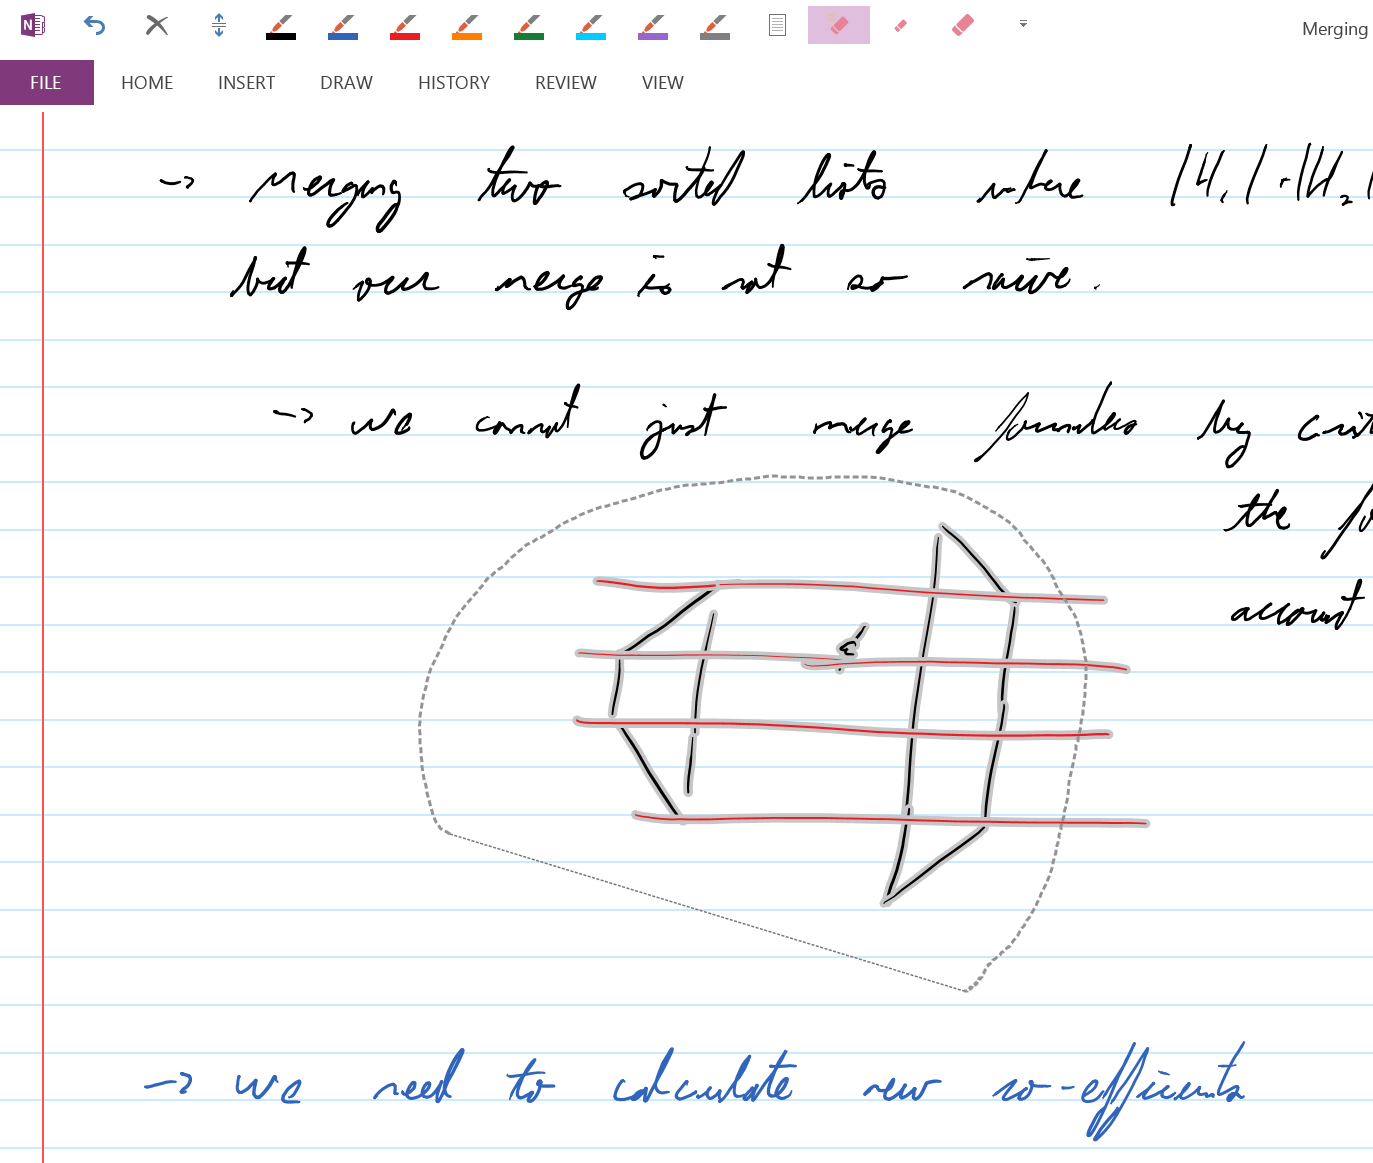
\includegraphics[width=0.50\textwidth]{figures/fig_onenote}
  \caption{An example of partial enclosure range searching in 
  Microsoft OneNote. The selected line segments are not entirely 
  enclosed in the query region.}
  \label{fig:intro:onenote}
\end{center}
\end{figure}

The paper proposes algorithms for the following variations of 
the partial enclosure range searching problem.  
\begin{description}
\item[\PERS{} - Partial enclosure range searching:] Here $S$ 
is a given a set of line segments, and the query object $Q$ 
is an axis-parallel rectangle or a slab bounded by two parallel 
lines of arbitrary orientation. The objective is to count 
the number of objects in $S$ that lie in $Q$. We have 
considered different combinations depending on the orientation 
of the line segments in $S$ and the orientation of the 
rectangle/slab $Q$.
\item[\PEAC{} - Partial enclosure area computation:] Here $S$ 
is a given convex/monotone/arbitrary polygon, and $Q$ is an 
axis-parallel rectangle/slab. The objective is to compute the 
area of the region $S\cap Q$. 
\end{description}

Table~\ref{tab:contributions} gives a broad overview of the 
proposed results in this paper. Here, `AP' is used for {\it 
Axis-Parallel}, `AO' for {\it Arbitrary Orientation}, and 
`P' for {\it Polygon}.

\begin{table}[t]
\caption{Summary of Contributions}
\label{tab:contributions}
\centering
\begin{tabular}{l l l l l l}
\hline \hline
Problem & Object & Query  & Space & Time & Query \\
\hline
\PERS{}& AP Segment & AP Rectangle  & $O(n\log^3n)$ & $O(n\log^3n)$ & $O(\log^3n$ \\
\PERS{} & AO Segment & AP Rectangle  & $O(n\log^7n)$ & $O(n\log^7n)$ & $O(\sqrt{n}\log^7n)$ \\
\PERS{} & AP Segment & AO Slab  & $O(n\log^2n)$ & $O(n\log^3n)$ & $O(\sqrt{n}\log^3n)$ \\
\PERS{} & AP Segment & 2 AO Slabs  & $O(n\log^3n)$ & $O(n\log^3n)$ & $O(\sqrt{n}\log^3n)$ \\
\PEAC{} & Convex P & Rectangle  & $O(n)$ & $O(n)$ & $O(\log n)$ \\
\PEAC{} & Convex P & Convex $k$-gon  & $O(n)$ & $O(n)$ & $O(k \log n)$ \\
\PEAC{} & Monotone P & AP Rectangle  & $O(n\log n)$ & $O(n\log n)$ & $O(\log n)$ \\
\PEAC{} & Monotone P & AP Rectangle  & $O(n)$ & $O(n\log n)$ & $O(\sqrt{n})$ \\
\PEAC{} & Simple P & Horiz Slab  & $O(n)$ & $O(n)$ & $O(\log n)$ \\
\hline
\end{tabular}
\end{table}


The next four sections of the paper cover partial enclosure 
range searching queries on successively more sophisticated 
geometric objects. Section~\ref{:rectangles} focuses the 
partial enclosure range counting problem when the objects 
are line segments and the query region is an axis-parallel 
rectangle, Section~\ref{:slabs} considers the counting problem 
in the same environment where the query region is an 
arbitrary-oriented slab. Section~\ref{:convexp} and Section 
\ref{:monotonep} consider the partial enclosure volume 
computation problem where the objects are respectively 
a convex polygon and a monotone polygon; in both cases, the 
query region is an axis-parallel rectangle. Finally, we 
conclude in Section~\ref{:conclusion}, where we summarize our 
contributions and future work. 

\section{PERS problem for Axis-Parallel Rectangles}
\label{:rectangles}


We present two variations of the \PERS{} problem in this section. 
In the first variation (Subsection~\ref{:rectangles:ap}), the line 
segments in $S$ will  be axis-parallel, whereas in the next variation 
(Subsection~\ref{:rectangles:ao}), we allow the segments in $S$ to have 
arbitrary orientation. In both the variations, the query rectangle $Q$ 
is axis-parallel. We first define the concept of partial enclosure of 
segments as follows:


\begin{definition}
A segment $s \in S$ is said to satisfy the {\em partial enclosure 
property} with respect to a query object $Q$ if and only if 
$|s \cap Q| \geq \rho \cdot |s|$, where $|x|$ denotes the length 
of the segment $x$ and $0 < \rho\leq 1$.
\end{definition}


%------------------------------------------------------------------------------
\subsection{Axis-Parallel Segments}
\label{:rectangles:ap}
In this section, we consider the following problem. 


\begin{problem}
Given a set $S$ of $n$ axis-parallel line segments in the plane, 
and a fixed parameter $\rho$ ($0 < \rho \leq 1$), we want to 
identify those segments which are sufficiently enclosed by 
an axis-parallel query rectangle $Q$ so as to satisfy the 
partial enclosure property. 
\end{problem}

We use the following notation. Each segment 
$s_i =(a_i, b_i, \ell_i) \in S$, $1 \leq i \leq n$ is defined 
by its left or bottom endpoints $(a_i, b_i)$ depending on whether 
$s_i$ is horizontal or vertical, and its length $\ell_i$. 
The query rectangle $Q$ is given by its bottom-left corner $(\alpha, 
\beta)$ and its top-right corner $(\gamma, \delta)$. \remove{Thus, its 
width is $w=\gamma-\alpha$.} We say that $s_i \in_\rho Q$ if and only 
if $s_i$ satisfies the partial enclosure property w.r.t. $Q$, 
otherwise $s_i \not \in_\rho Q$. 



\begin{figure}[t]
\centering
\includegraphics[width=1.00\columnwidth]{figures/fig_oo_cases}
\caption{An axis-parallel query on axis-parallel segments. Different cases 
of horizontal segments interacting with the query region are shown.}
\label{:fig:rectangles:ap:cases}
\end{figure}

For horizontal segments, we only need to consider the segments  
$s=(a, b, \ell)$
satisfying $\beta \leq b \leq \delta$. 
Figure~\ref{:fig:rectangles:ap:cases} illustrates several cases 
regarding how such a segment may interact with $Q$. 
Cases $(1)$, $(2)$, and $(3)$ demonstrate the cases where $s$ is 
entirely to the left, entirely within, or entirely to the right of $Q$, 
respectively. Case $(4)$ considers the situation where $s$ crosses 
only the left boundary of $Q$ (i.e., $\alpha \leq a+\ell \leq \gamma$). 
Depending on the partial enclosure parameter $\rho$, we further 
subdivide case $(4)$ into subcases $(4a)$ if $s \in_\rho Q$, and 
$(4b)$ if $s \not \in_\rho Q$. Cases $(5a)$ and $(5b)$ are similar 
to cases $(4a)$ and $(4b)$, but with respect to $\gamma$. Specifically, 
$s$ falls into case $(5a)$ or $(5b)$ when $\alpha \leq a \leq \gamma$ 
and $a+\ell > \gamma$. In case $(6)$, $s$ crosses both the left and right 
boundaries of $Q$, with neither of its endpoints inside $Q$;
the subcases are $(6a)$ if $s \in_\rho Q$ and $(6b)$ if $s \not 
\in_\rho Q$.
Our goal is to identify all segments belonging to cases $(2)$, $(4a)$, $(5a)$, 
and $(6a)$, and none of the segments belonging to any other case.

Let $w = \gamma - \alpha$ be the width of $Q$. We need to consider 
only the segments in $S_1 = \{s_i \in S \st \beta \leq b_i \leq \delta 
~\&~ \ell_i \leq \frac{w}{\rho}\}$, discarding all segments in case $(6b)$, 
among others.
We partition the members in $S_1$ 
according to the location of their left endpoint with respect to $\alpha$. 
Specifically, let $S_L = \{s_i \in S_1 \st a_i < \alpha\}$ and let 
$S_R = \{s_i \in S_1 \st a_i \geq \alpha\}$.
Now, we test an appropriate partial enclosure expression to determine 
whether $s_i$ should be counted. For segments in $S_L$, we want to 
ensure that ``not too much of $s_i$ is outside of $Q$'', i.e., $S_L' 
= \{ s_i \in S_L \st \alpha - a_i < (1 - \rho) \cdot l_i\}$.
For segments in $S_R$, we want to ensure that ``enough of $s_i$ is inside 
$Q$'', i.e., $S_R' = \{s_i \in S_R \st \gamma - a_i \geq  \rho l_i\}$.

\begin{observation}
The subset of segments satisfying the partial enclosure property is 
$S_\rho = S_L' \cup S_R'$. 
\end{observation}

The members in $S_L'$ can be identified by mapping each 
segment $s_i\in S$ to a point $\hat{s_i}=(b_i,\rho\cdot\ell_i,
a_i,a_i + (1-\rho) \cdot\ell_i)$ in $I\!\!R^4$, and then observing  
those points lying inside the  four dimensional query box 
$\hat{Q}=[\beta, \delta] \times (0,w] \times (-\infty,\alpha] \times 
(\alpha,\infty)$. 
Similarly, the members in $S_R'$ can be identified 
by mapping each segment $s_i\in S$ to a point 
$\hat{\hat{s_i}}=(b_i,\rho\cdot\ell_i,a_i,a_i + \rho 
\cdot\ell_i)$ in $I\!\!R^4$, and then observing  
those points lying inside the  four dimensional query box 
$\hat{\hat{Q}}$ = $[\beta, \delta] \times (0, w] \times [\alpha, \infty) 
\times (-\infty, \gamma]$.

We can answer these queries by constructing two 4D range 
trees~\cite{Deberg} with two sets of points 
$\{\hat{s_i}|s_i \in S\}$ and 
$\{\hat{\hat{s_i}}|s_i \in S\}$ respectively, and 
executing the counting query with the corresponding 4D query 
rectangle. The preprocessing time and space required for 
constructing these two range trees are both $\BigOh{n \log^3{n}}$, 
and the query can be answered in $\BigOh{\log^3{n}}$ time. Finally, 
we report the sum of two results as the answer of the query. 
Note that we can use the same first three levels for both the 
range trees since the first three components of both the types 
of query points (for $a<\alpha$ and $a > \alpha$) are same. In the  
third level, we create \emph{two} associated structures, one for 
each of the partial enclosure expressions, and query the one as 
needed. 

For vertical segments, the method of querying is exactly similar 
to that for horizontal segments, only we need to consider the 
height of $Q$ instead of its width, and we consider symmetric 
coordinates of each segment while mapping them to points in 4D. 
The following theorem summarizes the solution.

\begin{theorem}
\label{th:ap}
Given a set of $n$ axis-parallel line segments, we can identify a 
set of disjoint subsets containing all segments which satisfy the partial 
enclosure property for an axis-parallel query rectangle in $\BigOh{\log^3{n}}$ 
time,
with a data structure requiring $\BigOh{n\log^3{n}}$ preprocessing time and 
space.
\end{theorem}

%------------------------------------------------------------------------------
\subsection{Arbitrarily-Oriented Segments}
\label{:rectangles:ao}

In this subsection, we allow each segment $s_i \in S$ to have any 
arbitrary orientation. They may intersect among themselves. 
Here, the partial enclosure problem is stated as follows:

\begin{problem}
Given a set of $n$ arbitrarily-oriented line segments in the plane, and a 
fixed parameter $\rho$ such that $1/2 < \rho \leq 1$, we want to identify 
those segments which are sufficiently enclosed by an axis-parallel query 
rectangle $Q$ so as to satisfy the partial enclosure property. A segment 
$s$ satisfies this property if and only if $|s \cap Q| \geq \rho \cdot |s|$.
\end{problem}



We use $s_i= [(a_i,b_i), (c_i,d_i)]$ to denote a segment, where $(a_i,b_i)$ 
and $(c_i,d_i)$ are two end-points of $s_i$ satisfying $a_i\leq c_i$, 
and if $a_i = c_i$ then $b_i < d_i$. The problem statement is as 
follows.




\subsubsection{Decomposing the Problem}
\label{:rectangles:ao:approach}

We have three principal cases to consider:  those segments which 
have both endpoints inside $Q$,  those with only one endpoint inside 
$Q$, and  those with both endpoints outside $Q$ which still intersect $Q$.  

We first construct a 4D range tree $\cal T$ with the points $(a_i, b_i, c_i, 
d_i)$ 
for each $s_i \in S$, and execute a 4D range query with query box 
$[\alpha, \gamma] \times [\beta, \delta] \times [\alpha, \gamma] \times 
[\beta, \delta]$ corresponding to $Q=[\alpha,\beta] \times [\gamma,\delta]$ 
to identify all the segments satisfying the different cases. 
The first case, where both the end-points are inside $Q$, will all satisfy the 
partial enclosure property.

For the second case, we apply the same method, but on a {\it virtual} segment as 
follows. For each $s_i=
[(a_i,b_i),(c_i,d_i)] \in S$, create two virtual segments $s_i'$ and 
$s_i''$, where $s_i' \subseteq s_i$, $s_i'$ has an endpoint $(a_i,b_i)$, 
with $|s_i'| = \rho \cdot |s_i|$, and $s_i'' \subseteq s_i$, $s_i''$ 
has an endpoint $(c_i,d_i)$, with $|s_i''| = \rho \cdot |s_i|$. Thus, if 
$s_i' \in Q$ and/or $s_i'' \in Q$, then $s_i \in_\rho Q$. Counting both 
cases may double-count some 
segment(s) which have both endpoints in $Q$, so we subtract the count 
accordingly. 
As in the previous case, we can solve this case using a 4D range query.

The last case, where both the endpoints of a segment are outside $Q$, 
is the most challenging case to handle. We begin by partitioning the 
space outside $Q$ into 8 regions by extending lines through its 
horizontal and vertical boundaries. These regions are labelled as 
$I, II, \ldots, VIII$ in anticlockwise order starting from the 
left-middle region (see Figure~\ref{fig:rectangles:ao:regions}). Any 
segment which passes through $Q$ but has neither endpoint in $Q$ 
will have its endpoints in two distinct regions. Not every pair of 
regions is legal\footnote{For example, a segment with its two endpoints 
in regions $I$ and $II$ respectively, cannot intersect $Q$.}.

\begin{figure}[t]
\begin{center}
  \includegraphics[width=0.5\textwidth]{figures/fig_ao_regions}
  \caption{The 8 regions surrounding $Q$.}
  \label{fig:rectangles:ao:regions}
\end{center}
\end{figure}

A segment which passes through $Q$ may involve in any one of the following 
four classes depending on the pair of regions containing its two endpoints:

\begin{description}
\item[(i)] In two parallely opposite cells: $(I, V), (III, VII)$.
\item[(ii)] In two non-corner cells adjacent to a corner of $Q$: $(I, III), 
(III, V), (V,VII), (VII, I)$.
\item[(iii)] In a corner cell and a non-corner cell: $(II, V)$, $(II, VII)$, 
$(IV, I)$, 
$(IV, VII)$, $(VI, I)$, \newline $(VI, III)$, $(VIII, III)$, $(VIII, V)$.
\item[(iv)] In two corner cells: $(II, VI), (IV, VIII)$.
\end{description}

We will query for each class separately and combine our results at the end. 
In the first phase, we identify each class of problem 
by performing an appropriate rectangular range searching in the 
data structure $\cal T$. 
This also indicates which partial enclosure expressions we need to test in 
the second phase of the query. We develop expressions for each case below. 
In all the cases, we require the following additional definitions. Let 
$o_i = (e_i, f_i)$ be the mid-point of $s_i$. We use  
$d(u,v)$ to denote the Euclidean distance between two points $u,v \in 
\mathbb{R}^2$. Note that, for our choice of $\rho$, if $o_i \not\in Q$, 
then $s_i$ does not satisfy the partial enclosure property. Thus, we assume 
that 
$o \in Q$. we use $p'$ and $q'$ to represent the points of intersection of the 
segment 
$s$ with $Q$ closest to $p$ and $q$ respectively.

\begin{figure}[h]
\begin{minipage}[b]{0.5\linewidth}
\centering
\includegraphics[width=0.80\textwidth]{figures/fig_ao_case1}\\
(a)
\end{minipage}
\begin{minipage}[b]{0.5\linewidth}
\centering
\includegraphics[width=0.80\textwidth]{figures/fig_ao_case2}\\
(b)
\end{minipage}
\caption{Demonstration of (a) Case A and (b) Case B}
\label{fig:rectangles:ao:case12}
\end{figure}



%------------------------------------------------------------------------------
{\bf Class (i):}
This case deals with the segments that cross the parallel sides of $Q$. 
We present the details of the partial enclosure property for the subcase 
where $p=(a,b) \in I$ and $q=(c,d) \in V$; the solution for the subcase 
$(III, VII)$ is similar.

Assume for now that $o \in Q$. Let 
$p'$ and $q'$ be the points of intersection of the segment $s$ with 
$Q$ closest to $p$  and $q$ respectively. Let us draw a right angle 
triangle $\Delta p u o$ whose edge $[u,o]$ intersects the boundary 
of $Q$ at $u'=(\alpha, f)$. Similarly, the edge $[v,o]$ of  
$\Delta q v o$  intersects the boundary of $Q$ at 
$v' = (\gamma, f)$ (see Figure~\ref{fig:rectangles:ao:case12}(a)). 
The segment $s$ satisfies the partial enclosure property if 
$\frac{d(p, p') + d(q, q')}{d(p, q)} \leq 1 - \rho$. Let $L = \frac{d(p,q)}{2}$. By similarity 
of triangles $\Delta puo$ and $\Delta p'u'o$, we have
$\frac{d(p, p')}{d(p, o)} = \frac{d(p, p')}{L} = 
\frac{d(u, u')}{d(u, o)} = \frac{2 d(u, u')}{2 d(u, o)} = 
\frac{2(\alpha - a)}{c - a}$. Similarly, from the similarity of 
triangles $\Delta qvo$ and $\Delta q'v'o$, we have
$\frac{d(q, q')}{d(q, o)} = \frac{2(c - \gamma)}{c - a}$.

Thus, $\frac{d(p,p')+d(q,q')}{d(p,q)}=\frac{d(p,p')+d(q,q')}{2L} = 
\frac{1}{2} \left ( \frac{d(p,p')}{L} + \frac{d(q,q')}{L} \right ) 
 = \frac{\alpha - a}{c - a} + \frac{c - \gamma}{c - a} 
= 1 + \frac{\alpha - \gamma}{c - a}$. 

Therefore, the inequality $\frac{d(p, p') + d(q, q')}{d(p, q)} 
\leq 1 - \rho$ can instead be evaluated as $1 + \frac{\alpha - 
\gamma}{c - a} \leq 1 - \rho$, which is based on two query 
variables $\alpha$ and $\gamma$. We can further simplify the 
expression to $\rho(c - a) \leq \gamma - \alpha$, where the value 
of $\gamma - \alpha$ is a single query variable expression 
calculated at query time. This inequality can therefore be checked 
by augmenting the search tree $\cal T$ with another level with 
respect to the variable $h=\rho(c-a)$ corresponding to the segments 
in $S$, and querying with $h \leq \gamma-\alpha$ at the relevant 
nodes in that level of $\cal T$. Note that, if $o \not\in Q$, then 
$s$ does not satisfy the partial enclosure property, and this test 
will also fail. So, no test is required to check whether $q \in Q$.



%------------------------------------------------------------------------------
{\bf Class (ii)} This case is concerned with the segments which cross 
the mutually perpendicular sides of $Q$. We present the details 
of the partial enclosure property for the case where $p \in I$ 
and $q \in III$; the solutions for the other subcases  
are similar. 

Again let us assume that $o \in Q$ \footnote{If $o \not\in Q$, $s$ 
will not satisfy the partial enclosure property, and it can be shown 
that the test derived for this case will fail.}. 
As earlier, let $p'$ 
and $q'$ be the points of intersection of $s$ with the boundary of 
$Q$ closest to $p$ and $q$ respectively. As in Class (i), here also 
we draw the 
right-angle triangles $\Delta p u o$ and  $\Delta p'u'o$. In 
$\Delta p u o$, let $u' = (\alpha, f)$ be the point of intersection 
of the line segment $[u, o]$ with the boundary of $Q$, and 
$\Delta p'u'o$ is similar to $\Delta p u o$. Similarly, in 
$\Delta q v o$, the point $v' = (e, \beta)$ 
is the intersection point of $[v, o]$ with the boundary of $Q$, 
where $\Delta q' v' o$ is similar to $\Delta q v o$. See 
Figure~\ref{fig:rectangles:ao:case12}(b). We need to identify those 
segments satisfying $\frac{d(p, p')+d(q, q')}{d(p, q)} \leq 1-\rho$. 

By similarity of triangles, we have  $\frac{d(p, p')}{d(p, o)} = 
\frac{d(p, p')}{L} = \frac{d(u, u')}{d(u, o)} = \frac{2(\alpha - a)}
{c - a}$, and similarly, $\frac{d(q, q')}{d(q, o)} = \frac{2(\beta - d)}{b - 
d}$. 
Thus,
$\frac{d(p, p') + d(q, q')}{d(p, q)}=\frac{d(p, p') + d(q, q')}{2L} 
=\frac{1}{2} \left (\frac{d(p, p')}{L} + \frac{d(q, q')}{L} \right) 
= \frac{\alpha - a}{c - a} + \frac{\beta - d}{b - d}$.

Therefore, the inequality $\frac{d(p, p') + d(q, q')}{d(p, q)} 
\leq 1 - \rho$ can be tested by checking the equivalent inequality 
$\frac{\alpha - a}{c - a} + \frac{\beta - d}{b - d} \leq 1 - \rho$, 
defined on the two query variables $\alpha$ and $\beta$. On 
simplification, it becomes $\alpha + \beta \cdot \frac{c-a}{b-d} \leq 
\left ( (1 - \rho) + \frac{d}{b-d} \right ) \cdot (c-a) + a$.

Thus, we can map each segment $s$ satisfying Class (ii) to a point in the dual 
plane
given by
\[ (z,w)=
\left(\frac{c-a}{b-d}, \left ( (1 - \rho) + \frac{d}{b-d} \right ) \cdot (c-a) + 
a \right )
\]
The segments matching the 
partial enclosure expression correspond to the points satisfying the 
half-plane $y \geq \beta x + \alpha$ in the dual plane. In order 
to perform this test, we need to add a half-plane query data structure
(ham-sandwich cut tree) \cite{chan2012} with the points $(z,w)$ 
corresponding to the 
points in $S$ at the leaf level of $\cal T$ (independent of the arrangement 
made in Class (i)), and querying with the halfplane obtained from the query 
interval $Q$ as the desired node in the leaf level of $\cal T$. 

%------------------------------------------------------------------------------
{\bf Class (iii)}
Here, each segment has one endpoint in a corner region of $Q$, 
and the other endpoint in a non-corner region of $Q$ as shown in 
Figure~\ref{fig:rectangles:ao:case3}. We present the details of the partial 
enclosure property for the subcase where $p \in I$ and $q \in IV$; the 
solutions for other subcases of this case are similar.

\begin{figure}[t]
\begin{center}
  \includegraphics[width=0.45\textwidth]{figures/fig_ao_case3}
  \hspace{1.0em}
  \includegraphics[width=0.45\textwidth]{figures/fig_ao_case3b}
  \caption{Example of segments in  subcase $(I, IV)$ of class 
  (iii): the blue follows the proper handling, while the red shows the 
  incorrect handling.}
  \label{fig:rectangles:ao:case3}
\end{center}
\end{figure}

Consider the situation where $o \in Q$. We need to consider two 
subcases: (a) $s$ crosses the lines $x=\alpha$ and $y=\beta$ and 
(b) $s$ crosses the lines $x=\alpha$ and $x=\gamma$. See 
Figures~\ref{fig:rectangles:ao:case3}(a) and 
\ref{fig:rectangles:ao:case3}(b) for examples. Subcase (a) is very 
close to the example presented for class (ii). In that case, 
the only use of the fact that the endpoints of $s$ were located in 
regions $I$ and $III$ was to imply that $s$ crossed the lines 
$x=\alpha$ and $y=\beta$. As such, this subcase can use the same 
expression for testing the partial enclosing property for the segment 
$s$. Likewise, Subcase (b) is similar to the 
example presented for class (i) and can use exactly that expression 
for testing $s$.

Our initial query for identifying the regions of $p$ and $q$ does 
not allow us to differentiate between the subcases, so we will 
check both subcases simultaneously. From class (i) and class (ii), 
we have the following expressions:
$ \frac{\alpha - a}{c - a} + \frac{c - \gamma}{c - a} \leq 1 - \rho$
 and
$\frac{\alpha - a}{c - a} + \frac{\beta - d}{b - d} \leq 1 - \rho$
respectively. If $s$ belongs to subcase (a), then 
$\frac{c - \gamma}{c - a} \leq \frac{\beta - d}{b - d}$ since 
$\gamma$ is farther right than the point where $s$ exits from $Q$. 
Likewise, in subcase (b), 
$\frac{\beta - d}{b - d} \leq \frac{c - \gamma}{c - a}$.
Therefore, in either subcase, the result of the correct expression 
is larger than the incorrect one, allowing us to correctly reject 
segments by blindly checking both conditions. This also holds when 
$o \not \in Q$, since the expression for at least one subcase would 
exclude the segment.


% -----------------------------------------------------------------------------
{\bf Class (iv)}
This case is concerned with segments whose endpoints appear in 
diagonally opposite corner regions of $Q$. We present the details 
of the partial enclosure property for the case where $p \in II$ 
and $q \in VI$; the solution for subcase $(VI, VIII)$ is similar.

\begin{figure}[t]
\begin{center}
  \includegraphics[width=0.45\textwidth]{figures/fig_ao_case4a}
  \hspace{1.0em}
  \includegraphics[width=0.45\textwidth]{figures/fig_ao_case4b}

  \vspace{2.0em}
  
  \includegraphics[width=0.45\textwidth]{figures/fig_ao_case4c}
  \hspace{1.0em}
  \includegraphics[width=0.45\textwidth]{figures/fig_ao_case4d}

  \caption{Example of segments of subcase case $(II, VI)$ of class (iv): 
  in each figure, the blue lines show the proper handling.}
  \label{fig:rectangles:ao:case4}
\end{center}
\end{figure}

Assume for now that $o \in Q$. As in class (iii), here also we need to 
consider several subcases depending on which sides of $Q$ are 
intersected by $s$, namely (a) $s$ crosses the lines $x=\alpha$ and 
$y=\delta$, (b) $s$ crosses the lines $x=\alpha$ and $x=\gamma$, 
(c) $s$ crosses the lines $y=\beta$ and $y=\delta$, and (d)
$s$ crosses the lines $y=\beta$ and $x=\gamma$ (see Figure~
\ref{fig:rectangles:ao:case4} for examples of each subcase). 

Our query in the first phase for identifying the regions of $p$ and $q$ 
does not allow us to differentiate between subcases. However, 
it is sufficient to check all subcases simultaneously. The 
expression for subcase (b) comes directly from class (i).
Using similar techniques as we did for classes (i) and (ii), 
we develop the following set of partial enclosure expressions:

\begin{align*}
& (a) \quad \frac{\alpha - a}{c - a} + \frac{d - \delta}{d - b} \leq 1 - \rho
& (b) \quad \frac{\alpha - a}{c - a} + \frac{c - \gamma}{c - a} \leq 1 - \rho \\
& (c) \quad \frac{\beta  - b}{d - b} + \frac{d - \delta}{d - b} \leq 1 - \rho  
& (d) \quad \frac{\beta  - b}{d - b} + \frac{c - \gamma}{c - a} \leq 1 - \rho \\
\end{align*}

Subcases (b) and (c) can be simplified to orthogonal range 
queries, while in subcases (a) and (d), each segment needs to be mapped to 
a point in an appropriate plane and, as in class 
(ii), the halfplane counting query needs to be performed for answering 
the query problem. 

To illustrate that checking all four conditions simultaneously 
yields correct results, consider what happens if $s$ belongs 
to subcase (a), where $s$ crosses $\alpha$ and $\delta$. In 
these circumstances, $u'$ is above $\beta$, and we have that 
$\frac{\alpha - a}{c - a} \geq \frac{\beta - b}{d - b}$.  
Likewise, $v'$ is left of $\gamma$, so $\frac{d - \delta}{d - b} 
\geq \frac{c - \gamma}{c - a}$.  Therefore, the expression for 
(a) dominates the other expressions (i.e., $\text{(a)} \geq 
\text{(b)}$, $\text{(a)} \geq \text{(c)}$, and $\text{(a)} \geq 
\text{(d)}$), allowing us to identify qualifying segments for 
subcase (a) by blindly checking all conditions. This property 
is true for segments belonging to subcases (b), (c), and (d) 
as well. Furthermore, this test also holds when $o \not \in Q$, 
since the expression for at least one subcase would exclude the 
segment.


%------------------------------------------------------------------------------
\subsection{Construction and Analysis}
\label{:rectangles:ao:analysis}

Our method takes a very case-by-case approach to solving the problem, 
and executes in two phases. The first phase must classify segments 
belonging to one of the interesting classes among (i) to (iv), and then 
its appropriate subclass by searching the data structure $\cal T$.  
In the second phase, the partial enclosure property is tested by 
querying in the respective augmented data structures of $\cal T$ in 
its last level. 

Broadly, our solution to this problem uses a multi-level range tree 
\cite{Deberg} for the classification phase, and a combination of 
range trees and canonical subsets structures \cite{chan2012} to 
check the partial enclosure expressions. 

Identifying the segments which satisfy each case is a matter of 
testing a set of several conditions, all of which must be true. 
The order that we test the conditions in makes no difference to 
the correctness of the algorithm, but can have an impact on its 
space requirements. We now summarize the total time and space 
complexity for solving this problem. 

\paragraph{Class (i) - subcase $(p, q) \in (I, IV)$:}

We need to find those segments whose end-points are in the appropriate regions 
and satisfy the partial enclosure expression. For each $s_i \in S$, we construct 
a 5D 
point $v_i = (a_i, b_i, c_i, d_i, \rho(c_i - a_i))$. For the query, we construct 
a 5D box
$Q'= (-\infty, \alpha) \times [\beta, \delta] \times (\gamma, \infty) 
\times [\beta, \delta] \times (-\infty, \gamma - \alpha]$ and search for the 
points in the box. 
 The following lemma summarizes the complexity results. 

\begin{lemma}
\label{lem:ao:class1:v}
Given a set $S$ of $n$ line segments, we can identify the subset of $S$ 
belonging to class (i) \emph{and} satisfying the partial enclosure property 
in $\BigOh{\log^4{n}}$ time using a data structure requiring 
$\BigOh{n \log^4{n}}$ preprocessing time and space.
\end{lemma}

\paragraph{Class (ii) - subcase $(p, q) \in (I, III)$:} 
As with all cases, part of the problem involves first identifying those segments 
with endpoints in the appropriate regions.
In this case, however, the partial enclosure expression is evaluated using a 
half-plane query.

The classification portion is performed just as we have seen above. We map each 
segment to the 4D point $v_i = ( a_i, b_i, c_i, d_i )$.
For each $s_i \in S$, we define $h_i = \left ( \frac{c - a}{b - d}, \left ( (1 - 
\rho) + \frac{d}{b-d} \right ) \cdot (c-a) + a \right )$.
We need to construct a data structure which can answer queries on pairs $(v_i, 
h_i)$.
We can query the classification component using a range tree according to the 
following lemma.
\begin{lemma}
\label{lem:ao:class2:v}
Given a set of $n$ line segments, we can identify a set of disjoint subsets 
containing all segments belonging to class (ii) in $\BigOh{\log^3{n}}$ time 
using a data structure requiring $\BigOh{n\log^3{n}}$ preprocessing time and 
space.
\end{lemma}

By Theorem~\ref{th:chan}, we can query the half-plane component of our query 
objects using a canonical subsets data structure, giving the following lemma.

\begin{lemma}
\label{lem:ao:class2:h}
Given a set of $n$ line segments, we can identify a set of disjoint subsets 
containing all segments satisfying a half-plane representation of a partial 
enclosure expression in $\BigOh{\sqrt{n}\log{n}}$ time, using a data structure 
requiring $\BigOh{n\log{n}}$ preprocessing time and space.
\end{lemma}

Since the order that we check our conditions in does not affect correctness, we 
will check the half-plane condition first, then the endpoint classification.  
By Corollary~\ref{cor:multichan}, we can accomplish this by associating a 
classification structure with each subset of the half-plane structure. The 
resulting structure is summarized by the following lemma.

\begin{lemma}
\label{lem:ao:class2:c}
Given a set of $n$ line segments, we can identify a set of disjoint subsets 
containing all segments belonging to Class (ii) \emph{and} which satisfy their 
partial enclosure property in $\BigOh{\sqrt{n}\log^4{n}}$ time using a data 
structure requiring $\BigOh{n\log^4{n}}$ preprocessing time and space.
\end{lemma}


\paragraph{Class (iii) - subcase $(p, q) \in (I, IV)$:} 
This case can use the same orthogonal structure that we developed in 
Lemma~\ref{lem:ao:class1:v} and the same half-plane expression as in 
Lemma~\ref{lem:ao:class2:h}. 
One component of the query box needs to be updated to account for region IV, 
giving the following:
\[
(-\infty, \alpha) \times [\beta, \delta] \times (\gamma, \infty) \times 
(-\infty, \beta) \times (-\infty, \gamma - \alpha]
\]

By Corollary~\ref{cor:multichan}, we can combine these two data structures to 
create a new structure which can answer this case as summarized by the following 
lemma.

\begin{lemma}
\label{lem:ao:class3:c}
Given a set of $n$ line segments, we can identify a set of disjoint subsets 
containing all segments belonging to class (iii) \emph{and} which satisfy their 
partial enclosure property in $\BigOh{\sqrt{n}\log^5{n}}$ time using a data 
structure requiring $\BigOh{n\log^5{n}}$ preprocessing time and space.
\end{lemma}


\paragraph{Class (iv) - subcase $(p, q) \in (II, VI)$:} 
This case has the largest number of partial enclosure expressions which need 
checking, in addition to the usual endpoint classification step. 
As a result, it will be the largest data structure to build.

The basic steps are just as in the last three cases. 
To cover endpoint classification and the two orthogonal partial enclosure 
expressions, we will use a data structure and query box similar to 
Lemma~\ref{lem:ao:class1:v}, but extended to 6D to cover the extra partial 
enclosure expression.
We then apply Lemma~\ref{lem:ao:class2:h} and Corollary~\ref{cor:multichan} 
twice to handle the two half-plane partial enclosure expressions and associate 
the orthogonal range tree. 
The entire structure for this case is summarized by the following lemma.

\begin{lemma}
\label{lem:ao:class4:c}
Given a set of $n$ line segments, we can identify a set of disjoint subsets 
containing all segments belonging to Class (iv) \emph{and} which satisfy their 
partial enclosure property in $\BigOh{\sqrt{n}\log^7{n}}$ time using a data 
structure requiring $\BigOh{n\log^7{n}}$ preprocessing time and space.
\end{lemma}


\paragraph{Combining the Steps.} 

Querying the entire environment requires us to create the structures for 
handling the cases where one or both endpoints of a line segment lie entirely 
inside a query $Q$, as well as the structures for each of the cases when both 
endpoints lie outside of $Q$. 
Overall, this process is dominated by the structure required for the class (iv) 
segments. 
The following theorem summarizes the overall solution.

\begin{theorem}
\label{th:ao}
Given a set of $n$ arbitrarily-oriented line segments, we can identify a set of 
disjoint subsets containing all segments which satisfy the partial enclosure 
property for an axis-parallel query rectangle in $\BigOh{\sqrt{n}\log^7{n}}$ 
time, using a data structure requiring $\BigOh{n\log^7{n}}$ preprocessing time 
and space.
\end{theorem}



%\section{PERS problem for Arbitrarily-Oriented Slabs}
\label{:slabs}

In this section, we show how we can answer partial enclosure range searching 
query 
where the elements of $S$ are horizontal line segments, and the query region 
$Q$ 
is a slab bounded by two parallel lines of arbitrarily orientation. Next, we 
extend 
our solution for a query regions which is the intersection of two slabs. 

%------------------------------------------------------------------------------
\subsection{Querying with One Slab}
\label{:slabs:one}
In this section, we address the following problem. 
\begin{problem}
We are given a set $S$ of $n$ horizontal line segments in the 
plane, and a fixed parameter $\rho$ such that $0 < \rho \leq 1$. 
The objective is to identify those segments which are sufficiently 
enclosed inside (satisfy partial enclosure property with respect 
to) an arbitrarily oriented slab $Q$.
\end{problem}

As in Section \ref{:rectangles:ap}, here also we use a triple 
$s_i=(a_i,b_i,\ell_i)$ to represent an object in $S$. The 
query slab $Q$ is given by three inputs - $(\alpha, \beta, w)$,  
where the left and right bounding lines of $Q$ are defined by 
$L_1 : y = \alpha x + \beta$ and $L_2: y = \alpha x + \beta - 
\alpha w$ respectively. Thus, $w$ is the horizontal width of $Q$.

%------------------------------------------------------------------------------
\subsubsection{Identifying the Segments}
\label{:slabs:one:approach}
Identifying whether a segment $s_i \in_\rho Q$ (which satisfy the partial 
enclosure property), requires three broad steps:

\begin{enumerate}
\item Restrict segments to those which are ``not too long'' to fit 
sufficiently inside $Q$.
\item Classify all segments by whether their left endpoints are 
left or right of $L_1$.
\item For each class of segments, test an appropriate partial 
enclosure expression.
\end{enumerate}

We will use a multi-level canonical sets data structure 
\cite{chan2012} for answering these queries. 
We now describe the different steps of the query in more detail. 
Subsection~\ref{:slabs:one:analysis} describes the construction 
and analysis of the overall data structure.


%------------------------------------------------------------------------------
\subsubsection{Restrict Length}
%\label{:slabs:one:details:restrict}
The first step of the query is to perform a length test, as it 
simplifies future steps. With the query parameter $w$ given, 
only segments with length $\ell \leq \frac{w}{\rho}$ can satisfy 
the partial enclosure property. Thus, with a 1-dimensional 
orthogonal range to query we can extract a subset 
$S_1 = \{ s\in S \st \rho \ell \leq w \}$.


%------------------------------------------------------------------------------
\subsubsection{Classify Endpoints}
%\label{:slabs:one:details:classify}
The left endpoints of the members of $S$ can be in any one of the three 
regions: (1) left of $L_1$, (2) between $L_1$ and $L_2$, and (3) right 
of $L_2$. However, only those segments belonging to cases (1) and (2) 
are interesting to us. We will see that partitioning segments as left 
or right of $L_1$ is sufficient, as we can discriminate between cases 
(2) and (3) while testing partial enclosure expressions in the next step.

Identifying segments whose left endpoints appear to the desired side of 
$L_1$ can be accomplished using a half-plane query on the left endpoints 
of the members in $S$. Thus, we have $S_L = \{ s \in S_1 \st p \text{ is 
left of } L_1 \}$, and let $S_R = \{ s \in S_1 \st p \text{ is right of 
} L_1 \}$.


%------------------------------------------------------------------------------
\subsubsection{Check the Partial Enclosure Property}
%\label{:slabs:one:details:pep}
For each of $S_L$ and $S_R$, the final step is to identify those segments 
which satisfy the partial enclosure property.

\begin{figure}[h]
\begin{minipage}[b]{0.5\linewidth}
\centering
\includegraphics[width=0.60\textwidth]{figures/fig_aoq_left_l1}\\
(a)
\end{minipage}
\begin{minipage}[b]{0.5\linewidth}
\centering
\includegraphics[width=0.60\textwidth]{figures/fig_aoq_left_l2}\\
(b)
\end{minipage}
\caption{(a) Segments whose left endpoints are left of $L_1$, (b) Segments whose 
left endpoints are between $L_1$ and $L_2$.}
\label{fig:slabs:one:aoq_left_l1_l1l2}
\end{figure}

Set $S_L$ can be split into four parts as follows (see Figure 
\ref{fig:slabs:one:aoq_left_l1_l1l2}(a)).

\begin{itemize}
 \item[(1)] The entire segment is left of $L_1$ (which are not  counted),
 \item[(2)] The segment intersects $L_1$, and is sufficiently enclosed by $Q$,
 \item[(3)] The segment intersects $L_1$, but not sufficiently enclosed by 
 $Q$ (which are not counted),
 \item[(4)] The segment intersects both $L_1$ and $L_2$. 
\end{itemize}

Given a segment $s \in S_L$ with left endpoint $p = (a,b)$; $\iline{s}: y = b$ 
is the line through $s$. Let $(a', b)$ be the intersection point of $\iline{s}$ 
and $L_1$, where $a' = \frac{b - \beta}{\alpha}$. 

\begin{observation}\label{o21}
 $s \in_\rho Q$ if and only if $a' - a < (1 - \rho)\ell$.
\end{observation}
\begin{proof}
We look at each of the above cases to show that this single expression is 
enough 
to identify all segments correctly. 
First, the test directly identifies segments belonging to cases (2) or (3) 
since 
$a' - a$ is precisely the amount of $s$ outside of $Q$. 
This test rejects segments in case (1) since $a' - a > \ell
> (1-\rho)\ell$ and cannot satisfy partial enclosure property for any allowed 
value of $\rho$. 

Finally, this test is also sufficient for case (4) owing to the length 
restriction step, explained earlier. If a segment is not too far left 
of $L_1$, then either it crosses only $L_1$, and case (2) holds, or it 
crosses $L_1$ and $L_2$. In the latter case we know that $|s| < 
\frac{w}{\rho}$, where $w$ is the width of the query slab. Since any 
segment in case (4) has the property $|s \cap Q| = w$, this implies that 
$s \in_\rho Q$.
\end{proof}

Thus, among the segments in $S_L$, we can count the one satisfying the 
partial enclosure property by executing a halfplane range counting query:
$a' - a < (1 - \rho)\ell$ $\equiv$ $a + (1 - \rho)\ell > \frac{1}{\alpha} b - 
\frac{\beta}{\alpha}$. We map each segment $s$ to a point with coordinates 
$(b, a + (1-\rho)\ell)$. The segments in $S_L$ 
satisfying the partial enclosure expression then correspond to the points 
satisfying the half-plane $y > \frac{1}{\alpha}x - \frac{\beta}{\alpha}$.

%------------------------------------------------------------------------------

For the segments in $S_R$, we need to consider the following 
4 cases as shown in Figure \ref{fig:slabs:one:aoq_left_l1_l1l2}(b).



\begin{itemize}
 \item[(1)] The entire segment is between $L_1$ and $L_2$. Here, $s \in_\rho Q$.
 \item[(2)] The entire segment is right of $L_2$. Here $s \cap Q = \emptyset$, 
 and hence $s \not \in_\rho Q$.
 \item[(3)] The segment intersects $L_2$, and $s \in_\rho Q$.
 \item[(4)] The segment intersects $L_2$, but $s \not \in_\rho Q$.
\end{itemize}
Let $\iline{s}$ be the horizontal line through $s$, and $(a'', b)$ be the 
intersection point of $\iline{s}$ with $L_2$ where $a'' = \frac{b - 
\beta}{\alpha}
 + w$. The following observation is easy to show.
\begin{observation} 
$s \in_\rho Q$ if and only if 
 $a'' - a \geq \rho \ell$.
\end{observation}
As in the case of $S_L$, here also the counting of elements in $S_R$ 
satisfying $a'' - a \geq \rho \ell$, or equivalantly $\rho \ell + a 
\leq \frac{1}{\alpha} b - \frac{\beta}{\alpha} + w$, can be done using 
a half-plane range query. Here we map each segment $s=[(a,b),\ell]\in 
S_R$ to a point $(b, \rho \ell + a)$, and the query is performed with 
the halfplane  $y \leq \frac{1}{\alpha} x - \frac{\beta}{\alpha} + w$.

%------------------------------------------------------------------------------
\subsubsection{Construction and Analysis}
\label{:slabs:one:analysis}

We will use the multi-level canonical sets data structure described in 
Section~\ref{prelim} to perform parts of this query.
Each of the three steps given in subsection~\ref{:slabs:one:approach} will 
correspond to one nested level of the final data structure.
It is easiest to describe the structure inside-out, so we begin with the 
innermost structure.


%------------------------------------------------------------------------------

The innermost structure answers the length restriction step of the overall 
query. 
This is easily answered using a 1-dimensional range tree (AVL tree) 
\cite{Deberg}, 
keyed on the segment lengths. Thus, we have

\begin{lemma}
\label{lem:slabs:one:step1}
Given a set of $n$ horizontal line segments, we can identify a set of disjoint 
subsets containing all segments with length at most $\frac{w}{\rho}$ in 
$\BigOh{\log{n}}$ time, using a data structure of size $\BigOh{n}$, which can be 
built in $\BigOh{n \log{n}}$ preprocessing time.
\end{lemma}


% -----------------------------------------------------------------------------

To identify segments satisfying the partial enclosure property, we use the 
half-plane expressions as mentioned above. 
Two expressions we need to test, one for $S_L$ and the other for $S_R$. 
By Theorem~\ref{th:chan}, we can answer this type of half-plane query directly 
using a canonical subsets data structure, yielding the following lemma 
applicable to both cases.

\begin{lemma}
\label{lem:slabs:one:step2a}
Given a set of $n$ horizontal line segments, we can identify a set of disjoint 
subsets containing all segments which are not ``too much'' to one side of a 
query line in $\BigOh{\sqrt{n}\log{n}}$ time, using a data structure of size 
$\BigOh{n\log{n}}$, which can be built in $\BigOh{n\log{n}}$ preprocessing time.
\end{lemma}

With each subset created for this structure, we will associate the structure 
required for Lemma~\ref{lem:slabs:one:step1}.
Applying Corollary~\ref{cor:multichan} gives us the following result.

\begin{lemma}
\label{lem:slabs:one:step2b}
Given a set of $n$ horizontal line segments, we can identify a set of disjoint 
subsets containing all segments which are not ``too much'' to one side of a 
query line \emph{and} which do not exceed a maximum length in 
$\BigOh{\sqrt{n}\log^2{n}}$ time, using a data structure of size 
$\BigOh{n\log{n}}$, which can be built in $\BigOh{n\log^2{n}}$ preprocessing 
time.
\end{lemma}


% -----------------------------------------------------------------------------

We need to classify the left-endpoints of the segments as left or right of 
$L_1$. 
By Theorem~\ref{th:chan}, each of these queries can be answered by a canonical 
subsets data structure.
With each subset created by this structure, we will associate the structure from 
Lemma~\ref{lem:slabs:one:step2b}. 
Applying Corollary~\ref{cor:multichan} gives us the following result.

\begin{lemma}
\label{lem:slabs:one:step3}
Given a set of $n$ horizontal line segments, we can identify a set of disjoint 
subsets containing all segments whose left endpoints are to one side of a line, 
which are not ``too much'' to one side of a query line, \emph{and} which do not 
exceed a maximum length in $\BigOh{\sqrt{n}\log^3{n}}$ time, using a data 
structure of size $\BigOh{n\log^2{n}}$, which can be built in 
$\BigOh{n\log^3{n}}$ preprocessing time.
\end{lemma}


% -----------------------------------------------------------------------------
Finally, to fully answer any query $Q$, we need to preprocess two such data structures, 
choosing our expressions appropriately for the left and right cases.
During query time, we will query both structures and combine their results.
The following theorem summarizes the overall solution.

\begin{theorem}
\label{th:slabs:one}
Given a set of $n$ horizontal line segments, we can identify a set of disjoint 
subsets containing all segments which satisfy the partial enclosure property for 
an arbitrarily-oriented query slab in $\BigOh{\sqrt{n}\log^3{n}}$ time, using a 
data structure of size $\BigOh{n\log^2{n}}$, requiring $\BigOh{n\log^3{n}}$ 
preprocessing time.
\end{theorem}


%------------------------------------------------------------------------------
%------------------------------------------------------------------------------
\subsection{Querying with Two Slabs}
\label{:slabs:two}

In this subsection, we consider a generalization of the slab query, where 
the objects in $S$ are same as in Section \ref{:slabs:one}, and the  
query input are a pair of slabs; we are interested in those segments 
which satisfy the partial enclosure property with respect to their intersection.
Formally, the problem is stated as follows:

\begin{problem}
Given a set $S$ of $n$ horizontal line segments in the plane, a fixed parameter 
$\rho$ such that $0 < \rho \leq 1$, we want to identify those segments $s \in S$ 
that satisfy 
the partial enclosure property ($s \in_\rho Q$) with respect to a parallelogram 
$Q$, or in other words,  $|s \cap Q| \geq \rho \cdot |s|$.
\end{problem}

If the two slabs are orthogonal, then the query is with respect to a 
rectangle of arbitrary orientation.  
The overall approach is very similar to subsection~\ref{:slabs:one}, and the 
data structure we will build to answer these queries is again based on the 
canonical sets structure outlined in Section~\ref{prelim}.



Here the query parallelogram $Q$ is defined by the intersection of two slabs, $S_p$ 
and $S_n$, which have positive and negative slopes, respectively. See Figure 
\ref{fig:slabs:two:ds}.

\begin{figure}[t]
\begin{center}
  \includegraphics[width=0.70\textwidth]{figures/fig_ds_slabs}
  \caption{A query parallelogram $Q$ formed by the inputs $\alpha$, $\beta$, 
$w_p$,
  $\gamma$, $\delta$, and $w_n$.}
  \label{fig:slabs:two:ds}
\end{center}
\end{figure}

Specifically, a query is given as a 6-tuple $(\alpha, \beta, w_p, \gamma, 
\delta, 
w_n)$, where $\alpha > 0$, $w_p > 0$, $\gamma < 0$, and $w_n > 0$. With these 
inputs, we define:

\begin{itemize}
 \item[$S_p$:] a slab $(\alpha,\beta,w_p)$ with positive slope $\alpha$, whose 
left edge is defined 
 by the line $L_1 : y = \alpha x + \beta$, and the width is $w_p$. Thus, its 
right edge 
 is defined by $L_2 : y = \alpha (x - w_p) + \beta$.
 \item[$S_n$:] a slab $(\gamma,\delta,w_n)$ with negative slope $\gamma$, whose 
left edge is defined 
 by the line $L_3 : y = \gamma x + \delta$, and the width is $w_n$. Thus, its 
right edge 
 is defined by $L_4 : y = \gamma (x + w_n) + \delta$.
 \item[$Q$:] The parallelogram $S_p \cap S_n$.
\end{itemize}



% -----------------------------------------------------------------------------
\subsubsection{Identifying the Segments}
\label{:slabs:two:approach}

Just as in the single slab problem, identifying the segments $s_i \in_\rho Q$ 
is accomplished by classifying its endpoints by how they interact with 
the boundaries of $S_p$ and $S_n$ forming $Q$,  and then testing an appropriate 
partial enclosure expression. 

\begin{figure}[t]
\begin{center}
  \includegraphics[width=0.65\textwidth]{figures/fig_ds_wpwn}
  \caption[Decomposition of the query region $Q$.]{Decomposition of the query 
region $Q$. The orientation of $Q$ depends on the relative widths of the slabs 
which define it.}
  \label{fig:slabs:two:wpwn}
\end{center}
\end{figure}

% -----------------------------------------------------------------------------

The query $Q$ is decomposed into three regions, $Q_a$, $Q_b$, and $Q_c$, by 
extending horizontal lines through each vertex of $Q$.
$Q_a$ and $Q_c$ are triangular regions, while $Q_b$ is a parallelogram. 
$Q_a$ is always defined by $L_1$ on the left and $L_4$ on the right. 
Likewise, $Q_c$, is always defined by $L_3$ on the left and $L_2$ on the right. 
The definition of $Q_b$ depends on the overall orientation of $Q$, which depends 
on the relationship between $w_p$ and $w_n$.
Specifically, $Q_b$ is defined by $L_1$ and $L_2$ when $w_p < w_n$ and defined 
by $L_3$ and $L_4$ when $w_p > w_n$.
When $w_p = w_n$, $Q_b$ disappears.


\subsubsection{Endpoint Classification:}
Once we know the definitions of each region, we can proceed with endpoint 
classification.
The goal of this step is to identify which partial enclosure expression is 
appropriate to test with each line segment $s$ by considering the appropriate 
borders of $Q$ it interacts with. 
Each region has its left, center, and right classification zone, $Z_L$, $Z_C$, 
and $Z_R$, where the center zone is the query region itself.
Figure~\ref{fig:slabs:two:endpoint} gives an illustration; $Z_L$, $Z_C$, and 
$Z_R$ are coloured blue, green, and red, respectively.

\begin{figure}[t]
\begin{center}
  \includegraphics[width=0.80\textwidth]{figures/fig_ds_endpoint}
  \caption[Classification zones for $Q$.]{Classification zones for each region 
of $Q$. Each region has a left, center, and right zone, coloured blue, green, 
and red, respectively, where we may find segments which need further testing.}
  \label{fig:slabs:two:endpoint}
\end{center}
\end{figure}

For $Q_a$, $Z_L$ is aligned with the base of $Q_a$, and extends up $L_1$. 
$Z_R$ is also aligned with the base of $Q_a$, and extends up $L_4$.
Both of these zones are open away from $Q$.
The zones for $Q_c$ are symmetric, being aligned with the top of the region, and 
with $Z_L$ and $Z_R$ extending down $L_3$ and $L_2$, respectively.

For $Q_b$, the classification zones we use depend on the orientation of the 
region.
When $w_p < w_n$, $Z_L$ is aligned with the base of $Q_b$ and extends up $L_1$, 
while $Z_R$ is aligned with the top of $Q_b$ and extends down $L_2$.
Conversely, when $w_p > w_n$, $Z_L$ is aligned with the top of $Q_b$ and extends 
down $L_3$, while $Z_R$ is aligned with the bottom of $Q_b$ and extends up 
$L_4$.
The former case is what is illustrated in Figure~\ref{fig:slabs:two:endpoint}.
$Z_C$ is $Q_b$ itself, which we decompose into two triangular subzones so that 
all of our zones are triangular in nature.
During the query, any time that we consider $Z_C$ for $Q_b$, we will query both 
subzones and consider their union.

Any segment interacting with a particular query region must have its endpoints 
in one of 6 combinations of classification zones: $(Z_L, Z_L)$, $(Z_L, Z_C)$, 
$(Z_L, Z_R)$, $(Z_C,\allowbreak Z_C)$, $(Z_C, Z_R)$, or $(Z_R, Z_R)$. 
For a segment $s \in S$ with endpoints $p$ and $q$:
\begin{itemize}
\item If $p, q \in (Z_C, Z_C)$, then $s$ is entirely inside $Q$ and $s \in_\rho 
Q$.
\item If $p, q \in (Z_L, Z_L)$, or $p, q \in (Z_R, Z_R)$ then $s$ is entirely 
outside $Q$ and $s \not \in_\rho Q$.
\item Otherwise, $s$ crosses one or both boundaries of the query region and we 
need to test the appropriate partial enclosure expression.
\end{itemize}


\subsubsection{Partial Enclosure Property:}
We begin by examining $Q_a$ in detail.
Let $s \in S$ be a horizontal line segment and let $\iline{s}$ be the line 
through $s$, defined by the equation $y = b$.
Let $(a', b) = \iline{s} \cap L_1$ and $(a'', b) = \iline{s} \cap L_4$, be the 
intersection points of $\iline{s}$ with $L_1$ and $L_4$, respectively, then $a' 
= \frac{b - \beta}{\alpha}$ and $a'' = \frac{b - \delta}{\gamma} - w_n$.
We have three combinations of classification zones that need further testing.

For the $(Z_L, Z_C)$ case, we know that $s$ only crosses $L_1$.
We check that not too much of $s$ is outside of $Q_a$, giving the  partial 
enclosure expression: $a' - a < (1 - \rho)\ell$, or in other words, 
$b \frac{1}{\alpha} - \frac{\beta}{\alpha} < a + (1 - \rho)\ell$.

We can query for segments matching this expression by performing a 
half-plane query on an appropriate dual-space.
For this expression in particular, we map each segment $s$ to a dual-point with 
coordinates $(b, a + (1-\rho)l)$, and query with the half-plane $y > 
\frac{1}{\alpha} x - \frac{\beta}{\alpha}$.

For the $(Z_C, Z_R)$ case, we know that $s$ only crosses $L_4$. 
We check that enough of $s$ is inside $Q_a$, which gives the  partial enclosure 
expression: $a'' - a \geq \rho \ell$, or in other words, $b \cdot 
\frac{1}{\gamma} - \frac{\delta}{\gamma} - w_n \geq a + \rho \ell$.
 We can test this expression by mapping each segment $s$ to a 
dual-point with coordinates $(b, a + \rho l)$ and then querying with the 
half-plane $y \leq \frac{1}{\gamma} x - \frac{\delta}{\gamma} - w_n$.

Finally, for the $(Z_L, Z_R)$ case, we know that both endpoints of $s$ are 
outside of $Q_a$, so we only need to measure the width of $s \cap Q_a$.  
Specifically, we require that:
\[
\begin{split} 
a'' - a' &\geq \rho l \\
%
\frac{b - \delta}{\gamma} - w_n - \frac{b - \beta}{\alpha} &\geq \rho l \\
%
\frac{b}{\gamma} - \frac{\delta}{\gamma} - w_n - \frac{b}{\alpha} + 
\frac{\beta}{\alpha} &\geq \rho l \\
%
b \cdot \left ( \frac{1}{\gamma} - \frac{1}{\alpha} \right ) + \left ( 
\frac{\beta}{\alpha} - \frac{\delta}{\gamma} - w_n \right ) &\geq \rho l \\
%
\end{split}
\]

We can test this expression by mapping each segment $s$ to a 
dual-point with coordinates $(b, \rho l)$ and then querying with the following 
half-plane.
$
y \leq \left ( \frac{1}{\gamma} - \frac{1}{\alpha} \right ) \cdot x + \left ( 
\frac{\beta}{\alpha} - \frac{\delta}{\gamma} - w_n \right ).
$

Classification into the left and right zones is somewhat ``rough'', as 
the zone continues above $Q_a$ itself. 
This is not a problem in the $(Z_L, Z_C)$ and $(Z_C, Z_R)$ cases since one 
endpoint of $s$ is classified directly in the closed zone $Z_C$ and the segments 
are horizontal.
However, it can happen that a segment classified into $(Z_L, Z_R)$ is entirely 
above $Q_a$. 
In this case, since we are measuring $a'' - a'$, and $a'' < a'$ above the apex 
of $Q_a$, the expression will be negative and the segment will be rejected.

The partial enclosure expressions for $Q_b$ and $Q_c$ are developed using 
exactly the same reasoning as for $Q_a$, differing only by which of the lines 
$L_1$, $L_2$, $L_3$, and $L_4$ we use to define $a'$ and $a''$.


% -----------------------------------------------------------------------------
\subsubsection{Construction and Analysis}
\label{:slabs:two:analysis}

We will use a multi-level query structure for this problem, just as we did for 
the single slab query.
Each of the steps given in Section~\ref{:slabs:two:approach} will correspond to 
one nested level of the data structure.
It is easiest to describe the structure inside-out, so we begin with the 
innermost structure.

To identify segments satisfying a partial enclosure expression, we use the 
half-plane dual-spaces we developed in subsection~\ref{:slabs:two:approach}. 
By Theorem~\ref{th:chan}, we can answer such a half-plane query directly using a 
canonical subsets data structure, yielding the following lemma.

\begin{lemma}
\label{lem:slabs:two:step1}
Given a set of $n$ horizontal line segments, we can identify a set of disjoint 
subsets containing all segments which are not ``too much'' to one side of a 
query line in $\BigOh{\sqrt{n}\log{n}}$ time, using a data structure of size 
$\BigOh{n\log{n}}$, which can be built in $\BigOh{n\log{n}}$ time.
\end{lemma}

We need to be able to classify the right endpoints of our segments into any of 
the classification zones of each query region.
Each of these regions are triangular in nature and can be queried with a 
canonical subsets data structure. 
With each subset created by this structure, we will associate the structure from 
Lemma~\ref{lem:slabs:two:step1}. 
Applying Corollary~\ref{cor:multichan} gives us the following result.

\begin{lemma}
\label{lem:slabs:two:step2}
Given a set of $n$ horizontal line segments, we can identify a set of disjoint 
subsets containing all segments which have their right endpoint in a query 
triangle, and which are not ``too much'' to one side of a query line, in 
$\BigOh{\sqrt{n}\log^2{n}}$ time, using a data structure of size 
$\BigOh{n\log^2{n}}$, which can be built in $\BigOh{n\log^2{n}}$ time.
\end{lemma}


Next, we need to be able to classify the left endpoints of our segments into any of 
the classification zones as well, which will use another canonical subsets data 
structure.
With each subset of this structure, we continue to build up our multi-level 
structure by associating the structure from Lemma~\ref{lem:slabs:two:step2}. 
By applying Corollary~\ref{cor:multichan} again, we have the following.

\begin{lemma}
\label{lem:slabs:two:step3}
Given a set of $n$ horizontal line segments, we can identify a set of disjoint 
subsets containing all segments which have their left and right endpoints in 
given query triangles, and which are not ``too much'' to one side of a query 
line, in $\BigOh{\sqrt{n}\log^3{n}}$ time, using a data structure of size 
$\BigOh{n\log^3{n}}$, which can be built in $\BigOh{n\log^3{n}}$ time.
\end{lemma}


Finally, 
to fully answer a query $Q$, we only need one instance of the structures for 
classifying the left and right endpoints, since these structures can support all 
of the different triangular classification queries we need to perform.
We will need to preprocess several versions of the innermost level which 
determines the partial enclosure expression, however.
During query time, we check $(Z_C, Z_C)$, $(Z_L, Z_C)$, $(Z_C, Z_R)$ and $(Z_L, 
Z_R)$ for every query region. 
For any of the latter three zone combinations which are non-empty, we check the 
innermost structure corresponding to the appropriate partial enclosure 
expression.
The following theorem summarizes this process.

\begin{theorem}
\label{th:slabs:two}
Given a set of $n$ horizontal line segments, we can identify a set of disjoint 
subsets containing all segments which satisfy the partial enclosure property 
with respect to the intersection of two query slabs in 
$\BigOh{\sqrt{n}\log^3{n}}$ time, using a data structure of size 
$\BigOh{n\log^3{n}}$, requiring $\BigOh{n\log^3{n}}$ preprocessing time.
\end{theorem}


%------------------------------------------------------------------------------
%------------------------------------------------------------------------------
\subsection{Remarks on Arbitrarily-Oriented Segments}
\label{:slabs:remarks}

Our general approach can be extended to identify arbitrarily-oriented line 
segments which satisfy the partial enclosure property for one or two slabs, 
however, the resulting structure is very ``case heavy'' and involves a large 
number of query variables.

Arbitrarily-oriented segments can cross through the borders of $Q$ in many more 
ways than horizontal ones.
This prevents us from partitioning the environment into a simple set of 
classification zones, and increases the number of cases to consider.

The partial enclosure expressions for each case will also involve higher degree 
polynomials.
For example, a segment $s$ which crosses $L_1$ and $L_2$ has intersection points 
$p' = (a', b')$ with $L_1$ and $q' = (a'', b'')$ with $L_2$.  
To consider how much of the segment is inside the slab, we need to calculate the 
length of the segment from $p'$ to $q'$, as follows.
\[
\begin{split}
\|p'q'\|^2 
&= \left( \sqrt{(a'' - a')^2 + (b'' - b')^2} \right)^2 \\
%
&= (a'' - a')^2 + (b'' - b')^2 \\
%
&= (a'')^2 - 2a'a'' + (a')^2 + (b'')^2 - 2b'b'' + (b')^2
\end{split}
\]

Each term in the above expression represents several query variables when we 
consider the actual values for $a'$, $b'$, $a''$, and $b''$.  
Let $\iline{s}$ be the line through $s$, and assume that it is defined as $y = 
mx + t$, then
$a'  = \frac{\beta - t}{m - \alpha}$, 
$b'  = m \frac{\beta - t}{m - \alpha} + t$, 
$a'' = \frac{\beta - t - \alpha w}{m - \alpha}$ and  
$b'' = m \frac{\beta - t - \alpha w}{m - \alpha} + t$.

Multiplying and squaring these expressions to calculate $\|p'q'\|^2$ results in 
a high degree polynomial with respect to the number of independent query 
variable expressions.
The situation worsens when we consider intersections between $L_1$ or $L_2$ with 
$L_3$ or $L_4$, as we have to consider $\gamma$ and $\delta$ as well.
Such an expression \emph{can} be mapped to a high-degree half-space and then be 
queried with a canonical subset structure, but the space and query times suffer.


%\section{PEAC Problem on Convex Polygons}
\label{:convexp}

In this section, we consider the partial enclosure area computation 
problem on convex polygons. 
The main contribution of this section is a method to calculate the area of a convex polygon appearing within a query rectangle. 
With the enclosed area in hand, deciding on the partial enclosure property is straight-forward.


%------------------------------------------------------------------------------
\subsection{Problem Definition}
\label{:convexp:problem-definition}

\begin{problem}
We are given a convex polygon $P$ consisting of $n$ edges and a fixed parameter $\rho$ such that $0 < \rho \leq 1$. We want to determine whether at least $\rho \cdot \area{P}$ is enclosed by a query rectangle $Q$.
\end{problem}

Throughout this chapter we use the following definitions. The polygon $P$ is defined by its edges $E = e_1, e_2, \ldots, e_{n-1}, e_n$, given in clockwise order, where $e_n$ and $e_1$ share a vertex to close the polygon.  A \emph{chord} of $P$ is a straight line segment incident to two edges which partitions $P$ into two regions.

A query $Q$ is given by its lower-left and upper-right corners $(\alpha, \beta)$ and $(\gamma, \delta)$, respectively. See Figure \ref{fig:convexp:example} for an example.

\begin{figure}[t]
\begin{center}
  \includegraphics[width=0.50\textwidth]{figures/fig_cvp_example}
  \caption[A convex polygon $P$ and query box $Q$.]{The query region $Q$ formed by the inputs $\alpha$, $\beta$, $\gamma$,  $\delta$, and a convex polygon $P$.}
  \label{fig:convexp:example}
\end{center}
\end{figure}

We say that $P$ is sufficiently enclosed by $Q$ to satisfy the partial enclosure property if and only if $\area{Q \cap P} \geq \rho \cdot \area{P}$. 
Throughout this chapter we will assume that $Q$ is an axis-parallel rectangle for ease of discussion. 
In subsection~\ref{:convexp:remarks} we will show how to use our method even when relaxing some restrictions on $Q$.

%------------------------------------------------------------------------------
\subsection{Overview of the Algorithm}
\label{:convexp:approach}

To achieve a fast query time, our algorithm requires some preprocessing on $P$ to speed up certain area calculations. Before describing the preprocessing, we outline the query algorithm here.

\begin{enumerate}
 \item Identify which edges of $P$ are intersected by $Q$.
 
 \item Enumerate the intersecting edges in clockwise order to determine which areas of $Q$ are inside of $P$, and which are outside. There are at most 4 pairs of intersecting edges where $P$ crosses into $Q$, and subsequently back out.
 
 \item For each entrance/exit pair:
 \begin{enumerate}
  \item Consider the point $s$ on the entrance edge and the point $t$ on the exit edge where $P$ intersects the boundary of $Q$.
  The segment $st$ through the interior of $Q$ forms a \emph{chord} of $P$.
  
  \item On one side of $st$, we have the subpolygon $P_{st}$ defined by a subchain of $P$ (including some partial component of the entrance and exit edges) and the segment $st$ itself. 
  $P_{st} \subseteq Q$, so we must calculate its area as part of our overall query.
  
 \end{enumerate}

 \item Assuming that $P$ and $Q$ \emph{do} intersect, the assembled collection of all such entrance and exit points from the previous step, as well as any corners of $Q$ which are inside $P$ define $P_I$.
We can also think of this as the space on the ``insides'' of all the chords. 
$P_I$ is a polygon of not more than 8 edges. 
$P_I \subseteq Q$, so we must calculate its area as part of our overall query.
 
\end{enumerate}


% -----------------------------------------------------------------------------
\subsection{Preprocessing}
\label{:convexp:preprocessing}

In order to help with calculating the area of the subpolygons identified by step 3(b), above, we will preprocess the area of several chords of $P$, storing the results in a binary search tree $T_P$. 

A chord from edge $e_i$ to $e_j$, $i < j$, is defined as the segment through the interior of $P$ from the vertex of $e_i$ which is not shared with $e_{i+1}$ to the vertex of $e_j$ which is not shared with $e_{j-1}$.
For certain values of $i$ and $j$ (detailed below), we will calculate the area of the subpolygon defined by the chord segment itself and the edges $e_i, e_{i+1}, \ldots, e_j$.

In order to query chords between two edges $e$ and $e'$ where the sequence of edges includes $e_n$ (i.e., the edge sequence is of the form $e, \ldots, e_{n-1}, e_{n}, e_{1}, e_{2}, \ldots e'$), we double the edge list to $e_1, e_2, \ldots, e_{n-1}, e_{n}, e_{1}', e_{2}', \ldots, e_{n-1}', e_n'$ where $e_i = e_i'$ for $1 \leq i \leq n$.
Any chord query between two edges $e_i$ and $e_j$ where $j < i$ is instead queried as $e_i$ and $e_j'$.

Every node in $T_P$ records the extremal edges of a chord, and the area of that chord. Given the edge list defining $P$, $T_P$ is constructed as follows. 
Split the edge list $E$ into halves, $E_l$ and $E_r$, and recursively construct $T_l$ and $T_r$, respectively. Initialize $T_P$ as a new tree node. If $|E| = 1$, then set $l(T_P) = r(T_P) = E$, set the area $a(T_P) = 0$, and return $T_P$. Otherwise, set $l(T_P) = l(T_l)$ and $r(T_P) = r(T_r)$. 
Let $v_m$ be the vertex shared by $E_l$ and $E_r$, and let $v_l$ and $v_r$ be the vertices at the opposite ends of $E_l$ and $E_r$, respectively, from $v_m$. Then, $a(T_P) = \Delta v_l v_m v_r + a(T_l) + a(T_r)$.

The resulting tree can be built with only $\BigOh{n}$ preprocessing.
Each node $t$ of $T_P$ records the labels of the left and right edges of $P$ that it spans, and the total area of the subpolygon between those edges.
Given two edge labels $i$ and $j$, we can query $T_P$ and identify $\BigOh{\log{n}}$ subtrees between those labels which correspond to precalculated subpolygons.
This will not give us the total area of the subpolygon between any arbitrary $e_i$ and $e_j$, but it does reduce the problem significantly, as the remaining area to be calculated is bounded by a path of only $\BigOh{\log{n}}$ chords rather than $\BigOh{n}$ edges of $P$.

\begin{figure}[t]
\begin{center}
  \includegraphics[width=0.80\textwidth]{figures/fig_cvp_prep}
  \caption[Preprocessing the area of chords of $P$.]{Preprocessing the area of chords of $P$.  Each level forms a triangle with the chords of the previous level.}
  \label{fig:convexp:preprocessing}
\end{center}
\end{figure}


%------------------------------------------------------------------------------
\subsection{Locating Intersections}
\label{:convexp:intersections}

Following from the convexity of $P$, there can be at most $8$ intersections between $P$ and $Q$.
Each intersection can be found in the following way. 
Let $b_\alpha$ be the vertical boundary of $Q$ with $x$-coordinate at $\alpha$. 
Let $\iline{\alpha}$ be the vertical line through $b_\alpha$. 
Using a binary search on the edges of $P$, we can identify the edges $e_\alpha$ and $e_\alpha'$ which intersect $\iline{\alpha}$, if they exist, such that $e_\alpha$ is clockwise from $e_\alpha'$ along $P$.
Specifically, we test only the top chain of $P$ to find $e_\alpha$ and only the bottom chain of $P$ to find $e_\alpha'$.
We then determine if $e_\alpha$ and $e_\alpha'$ are intersected by the segment $b_\alpha$ itself by checking the $y$-coordinate of the intersection point. 
We will store a `nil' value with $e_\alpha$ and/or $e_\alpha'$ if the intersections do not exist or do not intersect $b_\alpha$.

Similarly, let $b_\gamma$ be the vertical boundary of $Q$ with $x$-coordinate at $\gamma$, and let $b_\beta$ and $b_\delta$ be the horizontal boundaries of $Q$ with $y$-coordinates at $\beta$ and $\delta$, respectively.  Using the same binary search technique on appropriate half-chains of $P$, we can collect $e_\beta$, $e_\beta'$, $e_\gamma$, $e_\gamma'$, $e_\delta$, and $e_\delta'$.  

If all of these values are nil, then $P$ does not intersect $Q$ at all, and one of the following is true:

\begin{itemize}
 \item $P \subset Q$, determined by selecting any edge of $P$ and checking whether it is contained in $Q$. This check takes $\BigOh{1}$ time.

 \item $Q \subset P$, determined by selecting any point $q \in Q$, projecting horizontal and vertical lines through $q$, and checking that the intersections of these lines with $P$ occur on opposite sides of $q$. This check takes $\BigOh{\log{n}}$ time.

 \item $P \cap Q = \emptyset$, determined to be true if the previous two tests are false.
\end{itemize}


% -----------------------------------------------------------------------------
\subsection{Chain Decomposition}

For the remainder of the query, we assume that $P$ and $Q$ \emph{do} intersect. 
Any intersections between them must come in pairs; i.e., if $P$ enters $Q$, it must leave elsewhere.
Our goal is to determine how $P$ and $Q$ interact, and then calculate the area of $P \cap Q$.  Figure \ref{fig:convexp:examples} shows some examples of how the two may interact.

\begin{figure}[t]
\begin{center}
  \includegraphics[width=1.00\textwidth]{figures/fig_cvp_examples}
  \caption{Examples of how $P$ and $Q$ may interact.}
  \label{fig:convexp:examples}
\end{center}
\end{figure}

Continuing to examine the problem in a clockwise direction, $P$ can enter $Q$ at $e_\alpha$, $e_\beta$, $e_\gamma$, and/or $e_\delta$.  Once $P$ enters $Q$, it must exit at one of $e_\alpha'$, $e_\beta'$, $e_\gamma'$, or $e_\delta'$ before any other entrance can occur.

We can find all entrance/exit pairs with the following steps.
\begin{enumerate}
 \item Consider the following clockwise ordering of the entrance and exit labels as a circular list: $e_\alpha$, $e_\delta'$, $e_\delta$, $e_\gamma'$, $e_\gamma$, $e_\beta'$, $e_\beta$, $e_\alpha'$.
 
 \item Starting anywhere in the list, scan for a non-nil entrance label (a non-prime edge).
 
 \item Find the subsequent non-nil exit label, by continuing to walk the list in circular order.
 
 \item Mark any corners of $Q$ which are bypassed by step 2 as outside of $P$. The corners which remain inside will be important later.
 
 \item We are finished when we visit a non-nil entry label for the second time.
\end{enumerate}

Figure \ref{fig:convexp:chord} shows an example. In the figure, $e_\beta$ is an edge that enters into $Q$, while $e_\delta'$ is the corresponding exit edge. Both $e_\alpha'$ and $e_\alpha$ are nil. The corners of $Q$ at $(\alpha, \beta)$ and $(\alpha, \delta)$ are outside of $P$ since we know $P$ entered $Q$ before $(\alpha, \beta)$, and therefore all corners of $Q$ must be outside until the next non-nil entrance label.

\begin{figure}[t]
\begin{center}
  \includegraphics[width=0.50\textwidth]{figures/fig_cvp_chord}
  \caption[A query $Q$ intersecting $P$ at points $s$ and $t$.]{A query $Q$ intersecting $P$ at points $s$ and $t$. The segment $st$ is a chord of $P$ through the interior of $Q$.}
  \label{fig:convexp:chord}
\end{center}
\end{figure}

For an entrance edge $e_i$ and exit edge $e_j$, let $s$ and $t$ be the intersection points of $e_i$ and $e_j$ with the boundary of $Q$, respectively. 
The segment $st$ partitions $Q$ into two parts and forms a chord of $P$.

Let $P_{st}$ be the subpolygon ``cap'' of $P$ defined by the segment $st$, the portion of $e_i$ from $s$ towards $e_{i+1}$, the edges $e_{i+1}, e_{i+2}, ..., e_{j-1}$, and the portion of $e_j$ from $e_{j-1}$ to $t$.
Since $P_{st} \subset Q$, we need to calculate its area.

We first check if $e_i = e_j$.
In that case, a single edge of $P$ has formed both the entrance and exit of $Q$, the chord $st$ is a subsegment of that edge, and the area of $P_{st}$ is 0.
Otherwise, $P_{st}$ is a convex polygon.
Using the preprocessed subpolygon areas stored in $T_P$, the chain of edges $e_{i+1}$ to $e_{j-1}$ can be decomposed into $\BigOh{\log{n}}$ preprocessed subpolygons whose total area is found in the tree.
The remaining region of $P_{st}$ for which we do not yet know the area is comprised of a path of $\BigOh{\log{n}}$ chords from $T_P$, the partial edges of $P_{st}$ up to $s$ and $t$, and the segment $st$.
This region is a convex polygon with $\BigOh{\log{n}}$ vertices and its area can be calculated in $\BigOh{\log{n}}$ time.

The above process is repeated for each entry and exit pair of intersections, giving at most four caps of $P$.
We still need to calculate the area to the inside of each chord (the side away from the chord's cap).
This interior area may also be defined in part by the edges and corners of $Q$. 

More precisely, let $P_I$ be the polygon defined by all of the intersection  points of $P$ with the boundary of $Q$ (e.g., the points $s$ and $t$ for each cap), as well as any corners of $Q$ which are inside $P$. $P_I \subset Q$ and is comprised of $\BigOh{1}$ vertices, all of which have been previously identified in earlier steps of the query. Its area can be calculated in $\BigOh{1}$ additional time.


%------------------------------------------------------------------------------
\subsection{Analysis and Remarks}
\label{:convexp:analysis}

Our method has a straight-forward analysis. 
Preprocessing is limited to the creation of $T_P$ which requires total preprocessing time of $\BigOh{n}$, since the merge step of the recursion requires only $\BigOh{1}$.
Our query method involves several steps, but each requires only $\BigOh{1}$ or $\BigOh{\log{n}}$ time. 
The following theorem and corollary summarize our overall approach.

\begin{theorem}
\label{th:convexp:area}
Let $P$ be a convex polygon consisting of $n$ edges. In $\BigOh{n}$ time and space, we can create a data structure which allows us to determine $\area{Q \cap P}$ in $\BigOh{\log{n}}$ time, for any axis-parallel rectangular query region $Q$.
\end{theorem}

\begin{corollary}
\label{cor:convexp:mp}
Let $P$ be a convex polygon consisting of $n$ edges, and let $0 < \rho \leq 1$ be a fixed parameter. With $\BigOh{n}$ time and space, we can determine if $\area{Q \cap P} \geq \rho \cdot \area{P}$ in $\BigOh{\log{n}}$ time for any axis-parallel rectangular query $Q$.
\end{corollary}

Our method is easily extended to allow a query rectangle with any orientation.
Nearly all of the steps involved in calculating the area are only concerned with edges of $P$ and intersection points of lines through the boundaries of $Q$.
The only place we use the axis-parallel property of $Q$ is in Section~\ref{:convexp:intersections} where we calculate those intersection points.

To allow $Q$ to be arbitrarily-oriented, we modify our intersection testing in the following way. 
During preprocessing, we calculate $c$, the centrepoint of $P$, which can be done in $\BigOh{n}$ time.
Let $\iline{l}$ be a line through any boundary of $Q$ and let $\iline{c}$ be the line perpendicular to $\iline{l}$ through the centrepoint of $P$.
The line $\iline{c}$ crosses the boundary of $P$ in two places, and, using a binary search on the edges of $P$, we can identify the edges $e_a$ and $e_b$ that $\iline{c}$ crosses.
These two edges divide $P$ into two chains, $E_{ab}$ and $E_{ba}$.
We can now perform a binary search on each of these chains looking for intersections with $\iline{l}$ (which may or may not cross $P$ at all).
Figure~\ref{fig:convexp:ao} illustrates this process.

\begin{figure}[t]
\begin{center}
  \includegraphics[width=0.60\textwidth]{figures/fig_cvp_ao}
  \caption{Locating the intersections of $P$ with an arbitrarily-oriented $Q$.}
  \label{fig:convexp:ao}
\end{center}
\end{figure}

Our method can also be extended to allow for querying by an arbitrary convex $k$-gon.
The number of intersections we have to locate increases to $\BigOh{k}$, as does the number of chords across $P$.
Otherwise, we use exactly the same preprocessing and general query method as for rectangles. 
We require $\BigOh{k \log{n}}$ time to find all intersection points between $P$ and $Q$ and to calculate the areas of each cap of $P$. 
A further $\BigOh{k}$ time is needed to calculate the area of $P_I$. 
The total query time for a convex $k$-gon is thus $\BigOh{k \log{n}}$.
The overall approach is summarized by the following corollary.

\begin{corollary}
\label{cor:convexp:karea}
Let $P$ be a convex polygon consisting of $n$ edges. In $\BigOh{n}$ time and space, we can create a data structure which allows us to determine $\area{Q \cap P}$ in $\BigOh{k \log{n}}$ time, for any convex $k$-gon query region $Q$.
\end{corollary}

Work by Czyzowicz \textit{et al.}\cite{DBLP:conf/cccg/CzyzowiczCU98} and then Iacono and Langerman\cite{IaconoL00} gives an alternate method for calculating the area of a convex polygon cut by a chord.
This method requires only $\BigOh{n}$ preprocessing time and space, and can answer area queries in $\BigOh{1}$ time.
We could use this method to reduce the time needed to find the area within each cap of $P$ to $\BigOh{1}$ with no increase in the cost of our preprocessing.
However, calculating the area of a rectangle still requires us to expend $\BigOh{\log{n}}$ time locating the points of intersection between $P$ and $Q$, so our overall query time remains unchanged.

%\section{PEAC Problem on Monotone Polygons}
\label{:monotonep}


In this section, we describe the partial enclosure range searching problem on 
monotone polygons. Formally, the 
problem is stated as follows:

\begin{problem}
We are given a monotone polygon $P$ consisting of $n$ vertices and a fixed 
parameter $\rho$ such that $0 < \rho \leq 1$. 
We want to determine whether at least $\rho \cdot \area{P}$ is enclosed by an 
axis-parallel query rectangle $Q$, where $area(P)$ is the area of the polygon $P$.
\end{problem}

The main contribution of this section is a method to calculate the area of a 
monotone polygon appearing within an axis-parallel query rectangle. 
Once the enclosed area is calculated, determining if the partial enclosure 
property is satisfied is straight-forward.

Throughout this section, we will use the following definitions.
The input is a polygon $P$ embedded in the plane which, without loss of 
generalization, is monotone with respect to the $x$-axis (i.e., from left to 
right). 
$P$ is defined by its vertices $v_1, v_2, \ldots, v_n$, where $v_n$ and $v_1$ 
share an edge to close the polygon.
A query $Q$ is given by its lower-left and upper-right corners $(\alpha, \beta)$ 
and $(\gamma, \delta)$, respectively. See 
Figure~\ref{fig:monotonep:query-example} for an example.

\begin{figure}[t]
\begin{center}
  \includegraphics[width=0.50\textwidth]{figures/fig_mono_query}
  \caption[A monotone polygon $P$ with query $Q$.]{A monotone polygon $P$ with 
query $Q$. The area of $P$ enclosed by $Q$, $Q \cap P$, is highlighted.}
  \label{fig:monotonep:query-example}
\end{center}
\end{figure}


%------------------------------------------------------------------------------
\subsection{A First Problem}
\label{:monotonep:approach}

We will first describe an algorithm which solves a simpler problem, and then 
extend that solution into one for our main problem.

\begin{problem}
Given a monotone polygon $P$, and a query in the form of a horizontal slab $S$, 
what is the total area of $P$ enclosed by $S$?  i.e., what is $\area{S \cap P}$?
\end{problem}

Our overall approach for this problem is to define a function (actually, a 
collection of functions) which returns the area below a given horizontal query 
line. 

% -----------------------------------------------------------------------------
\subsubsection{Decomposing $P$}
\label{sec:decompose}

In order to create an area formula for the entire polygon, we decompose $P$ into 
a linear number of regions and calculate area formulas for each. These regional 
formulas are then combined into an overarching \emph{multi-region formula}.

We begin by sorting all of the vertices by their $x$-coordinates. 
If two vertices share the same $x$-coordinate (no more than two can do so, since 
$P$ is monotone), we can skip the duplicate without any other change to the 
algorithm. 
However, for ease of discussion, we will assume that every vertex has a distinct 
$x$-coordinate.
For the remainder of this section, we relabel the $x$-coordinates by their 
sorted order so that $x_1$ is the $x$-coordinate of the leftmost vertex of $P$, 
$x_2$ the next leftmost, etc.

Let $\iline{x}$ be the vertical line through any $x$-coordinate, and let $P_U$ 
and $P_L$ be the upper and lower chains of $P$, respectively. Consider the 
sequence of lines $\iline{x_1}, \iline{x_2}, \ldots, \iline{x_n}$ through the 
vertices of $P$.
For every line $\iline{x_i}$, let $a_i = \iline{x_i} \cap P_U$ and $a_i' = 
\iline{x_i} \cap P_L$ be the intersections of $\iline{x_i}$ with the upper and 
lower chains of $P$, respectively.

We will calculate all of these intersections as we walk from left to right over 
both $P_U$ and $P_L$ simultaneously. 
We also keep track of $e_i$ and $e_i'$, the edges of $P_U$ and $P_L$, 
respectively, which are intersected by $\iline{x_i}$, and upon which reside the 
points $a_i$ and $a_i'$. 
Where $\iline{x_i}$ intersects a vertex of $P_U$ or $P_L$, we store the edge to 
the right of that vertex as the corresponding value of $e_i$ or $e_i'$.
This walk allows us to generate a sequence of regions $R_1, R_2, \dots, R_{n-1}$ 
which have the following, equivalent definitions.
\begin{itemize}
 \item For each $1 \leq i \leq n - 1$, let $X_i$ be the vertical slab between 
$\iline{x_i}$ and $\iline{x_{i+1}}$, then $R_i = X_i \cap P$.

 \item $R_i$ is the area of $P$ bounded by the vertical segments $\iline{x_i} 
\cap P$ and $\iline{x_{i+1}} \cap P$ to the left and right, 
 and some portion of the edges $e_i$ and $e_i'$ to the top and bottom. 
 %(while, in general, $e_i$ and  $e_i'$ extend beyond $\iline{x_i}$ and 
$\iline{x_{i+1}}$, this excess is irrelevant to the definition of $R_i$).
 
 \item $R_i$ is the polygon formed by the cycle on $a_i, a_{i+1}, a_{i+1}', 
a_i'$.
\end{itemize}

 
Thus, each region is a (possibly degenerate) trapezoid.


% -----------------------------------------------------------------------------
\subsubsection{Area of a Region}
\label{sec:region_area}

For each region $R_i \in \{R_1, R_2, \ldots R_{n-1}\}$, we create a function 
$F(R_i, h)$ which will return the area of $R_i$ below a 
horizontal query line having a $y$-component of $h$.
Figure \ref{fig:monotonep:trapezoid} shows an example region.
From bottom to top, we can identify at most 4 ``critical heights'', where the 
nature of how the area of a region grows with respect to $h$ changes.
For a general region $R$, these 4 critical heights are:

\begin{figure}[t]
\begin{center}
  \includegraphics[width=0.1\textwidth]{figures/fig_mono_trap}
  \caption[A trapezoidal region of $P$.]{A trapezoidal region of $P$ for which 
we can derive an area function dependant on $h$.}
  \label{fig:monotonep:trapezoid}
\end{center}
\end{figure}

\begin{itemize}
\item $h_0$, where $R$ begins.
\item $h_1$, where $R$ stops growing as a triangle and begins growing as a 
rectangle.
\item $h_2$, where $R$ stops growing as a rectangle and begins growing as the 
base trapezoid of a triangle.
\item $h_3$, where $R$ ends.
\end{itemize}

These 4 critical heights give rise to a piecewise function representing the 
area, defined as follows.
\[
F(R, h) = \begin{cases}
0                  & \text{if }          h < h_0 \\
A(h')^2            & \text{if } h_0 \leq h < h_1 \text{ for } h' = h - h_0 \\
Bh' + C            & \text{if } h_1 \leq h < h_2 \text{ for } h' = h - h_1 \\
A'(h')^2 + C'      & \text{if } h_2 \leq h < h_3 \text{ for } h' = h_3 - h \\
C''                & \text{if } h_3 \leq h \\
\end{cases}
\]


In essence, the area function is a quadratic one, although, for different values 
of $h$, some or all of the coefficients are 0. The details of each part of this 
function, and the definitions of the constants $A, A', B, C, C'$ and $C''$ are 
as follows.

\begin{enumerate}
\item When $h < h_0$, the area of $R$ below $h$ is 0, since no part of $R$ 
exists below that measure.

\item When $h_0 \leq h < h_1$, the area of $R$ below $h$ grows as a triangle. 
Let $h' = h - h_0$.
The angle $\theta'$ between $e_i'$ and the vertical can be calculated as 
\[ 
\tan(\theta') = \frac{x_{i+1} - x_i}{h_1 - h_0}
\]

Let $t'$ be this ratio, then at $h'$, the base of the triangle has width $h' 
\cdot t'$. The area of the triangle is therefore $\frac{1}{2} (h')^2 t'$ and we 
set the constant $A = \frac{1}{2} t'$.

\item When $h_1 \leq h < h_2$, the area of $R$ includes all of the area between 
$h_0$ and $h_1$, which we store as the constant $C$.
The remaining area of $R$ up to $h$ grows as a rectangle.
Let $h' = h - h_1$, then the rectangular area is $(x_{i+1} - x_i)\cdot h'$, and 
we define the constant $B = (x_{i+1} - x_i)$.
Thus, the total area of $R_i$ up to $h'$ is $Bh' + C$.

\item When $h_2 \leq h < h_3$, the area of $R$ includes all of the area between 
$h_0$ and $h_2$, which we store as the constant $C_a'$.
The remaining area of $R$ up to $h$ grows as the base trapezoid of a triangle.
Let $h' = h_3 - h$ (note that this definition is somewhat reversed from the 
other cases).
We can calculate this area by taking the total area of the triangle, and 
subtracting the area of the triangle from $h_3$ down to $h$.  

The overall triangle between $h_2$ and $h_3$ has area 
\[ 
a = \frac{1}{2} \cdot (h_3 - h_2) \cdot (x_{i+1} - x_i) 
\]

The angle $\theta$ between $e_i$ and the vertical can be calculated as
\[ 
\tan(\theta) = \frac{x_{i+1} - x_i}{h_3 - h_2}
\]

Let $t$ be this ratio, then the smaller triangle from $h_3$ down to $h$ can be 
calculated as in case 2, giving $a' = \frac{1}{2}(h')^2 t$. 
The overall area from $h_2$ up to $h$ is then
\[ 
\begin{split}
a - a' &= \frac{1}{2} \cdot (h_2 - h_3) \cdot (x_{i+1} - x_i) - 
\frac{1}{2}(h')^2 t \\
%
\end{split}
\]

This expression is of the form $C_b' + A'(h')^2$.
Thus we set the constants $A' = -\frac{1}{2}t$, $C_b' = \frac{1}{2} \cdot (h_2 - 
h_3) \cdot (x_{i+1} - x_i)$, and $C' = C_a' + C_b'$ to complete the formula for 
this part of $F(R, h)$.

\item When $h_3 \leq h$, the total area of $R$ should be reported, which we 
store in $C''$.

\end{enumerate}

% -----------------------------------------------------------------------------
\subsubsection{Creating Multi-Region Formulas}
\label{sec:mr_formula}

After completing the previous step, we have a set of regions, and their area 
formulas, $R_i$ and $F(R_i, h)$ respectively for $1 \leq i \leq n-1$.
To complete the preprocessing for the horizontal slab query, we will process our 
regional area formulas into a list of multi-region formulas which can report the 
area of the entire polygon under a query line.

We begin by collecting tuples of all of the critical heights from our regional 
formulas. 
For every region $R_i$, we collect $(y, R)$ for $y \in \{h_0, h_1, h_2, h_3\}$ 
and $R = R_i$.
Let $\mathcal{Y}$ be the list of all such tuples across all regions, sorted by 
$y$-values from lowest to highest.

If we suppose for a moment that each $y$-value is distinct, then for each one 
there is exactly one region $R$ which is transitioning from one phase of growth 
to another.
That is, looking at the piecewise function $F(R, h)$ which determines the area 
of $R$ below a query line, a new piece of that function is taking over.
To create the multi-region formula for a new critical height, we copy the 
formula for the predecessor height (the lowest $y$-value starts with a formula 
set to 0).
To update the multi-region formula, we subtract the coefficients of $R$ for its 
previous phase of growth so that they no longer influence the formula, and then 
add the coefficients for the new phase.

Since neighbouring regions share vertices, the $y$-values will not be distinct.
Instead, several $y$-values will be collapsed into a single critical height in 
the list of multi-region formulas, with all appropriate constants from 
contributing regions added or subtracted as necessary.
Algorithm \ref{alg:monotonep:mf} gives the details of this process more 
formally.

\begin{algorithm}[h]
\LinesNumbered
\DontPrintSemicolon
\caption{BuildMultiRegionFormula}
\label{alg:monotonep:mf}
\SetKwFunction{fSort}{sort}
\KwIn{List of regions $\mathcal{R} = R_1, R_2, \ldots, R_{n-1}$}
\BlankLine
Initialize a list $\mathcal{Y}$\;
\ForEach{$R$ in $\mathcal{R}$}
{
$\mathcal{Y} \gets \mathcal{Y} \cup \{ (y,R) \;|\; y \in \{R.h_0, R.h_1, R.h_2, 
R.h_3\}\}$\;
}
\fSort{$\mathcal{Y}$ on $y$}\;
\BlankLine
$y' \gets $ minimum $y$-value in $\mathcal{Y}$\;
$F(P, y') \gets $ coefficients $A,B,C$ set to 0\;
\BlankLine
\ForEach{$(y, R)$ in $\mathcal{Y}$}
{
$F(P, y) = F(P, y')$\;
$i \gets \{0,1,2,3\}$ such that $y = h_i \in \{R.h_0, R.h_1, R.h_2, R.h_3\}$\;
\If{$i > 0$}{
$F(P,y).A \gets F(P,y).A - R.h_{i-1}.A$\;
$F(P,y).B \gets F(P,y).B - R.h_{i-1}.B$\;
$F(P,y).C \gets F(P,y).C - R.h_{i-1}.C$\;
}
$F(P,y).A \gets F(P,y).A + R.h_i.A$\;
$F(P,y).B \gets F(P,y).B + R.h_i.B$\;
$F(P,y).C \gets F(P,y).C + R.h_i.C$\;
\BlankLine
$y' \gets y$\;
}
\BlankLine
$H \gets $ the list of all $F(P, h)$ created above\;
\KwRet{$H$}
\end{algorithm}

The output of this algorithm is the list $H$ of multi-region formulas. Since 
$\mathcal{Y}$ was sorted by $y$-value, $H$ will be as well.


% -----------------------------------------------------------------------------
\subsubsection{Querying Multi-Region Formulas}
\label{:monotonep:query-mf}

We are now ready to query horizontal slabs against $P$. 
Let $F(P,h)$ be the multi-region area function for $P$, which is essentially a 
piecewise function given by Algorithm \ref{alg:monotonep:mf} in the form of 
a sorted list $H$.
Given two horizontal lines $\iline{\beta}$ and $\iline{\delta}$ defining our 
query slab, which have $y$-components $\beta$ and $\delta$, respectively with 
$\beta \leq \delta$, our query is answered as follows:

\begin{enumerate}
\item Our query parameter $\beta$ will not generally correspond to a critical 
height in $H$.
Perform a binary search on $H$ to find the formula stored with the 
\emph{predecessor} of $\beta$.
Denote this formula as $F_\beta$.
Evaluating $F_\beta(P, \beta)$ tells us the area of $P$ below $\beta$.

\item For $\delta$, we perform another binary search on $H$ to find $F_\delta$ 
such that $F_\delta(P, \delta)$ tells us the area of $P$ below $\delta$.

\item We can now calculate the area inside the query slab as
$F_\delta(P, \delta) - F_\beta(P, \beta)$.

\end{enumerate}

 
We summarise our results in the following theorem.

\begin{theorem}
\label{th:montonep:slab-area}
Let $P$ be a monotone polygon consisting of $n$ vertices. In $\BigOh{n \log{n}}$ 
time and $\BigOh{n}$ space, we can create a data structure that allows us to 
determine $\area{S \cap P}$ in $\BigOh{\log{n}}$ time for any horizontal slab 
query region $S$.
\end{theorem}



% -----------------------------------------------------------------------------
% -----------------------------------------------------------------------------
\subsection{Extending to Rectangular Queries}
\label{:monotonep:rect}

Our actual query, as introduced in Figure \ref{fig:monotonep:query-example}, is 
a rectangular area. Our solution to this type of query is extended from the 
methods we used to solve a horizontal slab query.

\subsection{Preprocessing}
\label{:monotonep:rect:pre}

We develop a list of regions $\mathcal{R} = R_1, R_2, \ldots, R_{n-1}$ just as 
in Section \ref{sec:decompose}.  Now, instead of constructing a single list of 
multi-region formulas to cover all of $P$, we will construct a tree of such 
lists so that for any $1 \leq i \leq j \leq n-1$, we can query the subpolygon 
$\bigcup_{k=i}^{j}{R_k}$ for its area below a query line $h$ in 
$\BigOh{\log{n}}$ time.

Let this multi-region formula tree be $T$; we construct $T$ in the following 
way. First, construct the multi-region formula tree for each half of the regions 
recursively, giving the subtrees $T_l$ and $T_r$. If $|\mathcal{R}| = 1$ for any 
recursive step, we create a leaf and return the area formula for that single 
region.

Let $H(T_l)$ and $H(T_r)$ be the multi-region formula lists for $T_l$ and $T_r$, 
respectively. 
We need to create a merged list, $H(T)$ representing the regions of both 
subtrees together. 
Unfortunately, we cannot just naively merge the formulas into a combined sorted 
list as each formula is only concerned with the regions upon which it was 
originally created. 

Instead, we need to generate new coefficients for each critical height of $h$ 
which will be valid for all regions of the combined area.
This process is precisely Algorithm \ref{alg:monotonep:mf} \emph{without} the 
initial sorting step, which we can avoid since $H(T_l)$ and $H(T_r)$ are already 
sorted.
Thus, we can build $H(T)$ in time $\BigOh{|H(T_l)| + |H(T_r)|}$.
Algorithm \ref{alg:monotonep:bmft} gives more formal details.

\begin{algorithm}
\LinesNumbered
\DontPrintSemicolon
\caption{BuildMultiRegionFormulaTree}
\label{alg:monotonep:bmft}
\SetKwFunction{fSort}{sort}
\SetKwFunction{fBMFT}{BuildMultiRegionFormulaTree}
\KwIn{List of regions $\mathcal{R} = R_1, R_2, \ldots, R_{n-1}$}
\BlankLine
\If{$|\mathcal{R}| = 1$}{
$T \gets $ create new leaf node\;
$H(T) \gets F(R,h)$\;
\KwRet{$T, H(T)$}
}
$m \gets \floor{\frac{|\mathcal{R}|}{2}}$\;
$\mathcal{R}_l = \{ R_1, R_2, \ldots, R_m \}$\;
$\mathcal{R}_r = \{ R_{m+1}, R_{m+2}, \ldots, R_{n-1} \}$\;
$T_l, H(T_l) \gets $ \fBMFT{$R_l$}\;
$T_r, H(T_r) \gets $ \fBMFT{$R_r$}\;
$T \gets $ Create new node with left child $T_l$ and right child $T_r$\;
$H(T) \gets $ Merge $H(T_l)$ and $H(T_r)$ using 
Algorithm~\ref{alg:monotonep:mf}\;
\BlankLine
\KwRet{$T, H(T)$}
\end{algorithm}

In the last step of the algorithm we create a list of formulas over all regions, 
which implies that we can answer horizontal slab queries from the root of $T$. 
Recursing on half of the regions at each step gives us a tree which will be 
balanced with depth $\BigOh{\log{n}}$. 
At each level of $T$, every critical height for every region is considered, 
resulting in $\BigOh{n}$ area formulas.
As mentioned, the merging step at each node is completed in linear time with 
respect to the number of regions processed. 
Therefore, the total time and storage required to build $T$ is 
$\BigOh{n\log{n}}$.  


% -----------------------------------------------------------------------------
\subsubsection{Querying}
\label{:monotonep:rect:querying}

\begin{figure}[t]
\begin{center}
  \includegraphics[width=0.50\textwidth]{figures/fig_mono_extra}
  \caption[Details of a query on a monotone polygon.]{A monotone polygon $P$ 
with query $Q$. The tiled areas cannot be queried using preprocessed area 
formulas and will require special handling.}
  \label{fig:monotonep:extra}
\end{center}
\end{figure}

Our query rectangle $Q$ is given by the lower-left and upper-right coordinates 
$(\alpha, \beta)$ and $(\gamma, \delta)$, respectively. We define 
$\iline{\beta}$ and $\iline{\delta}$ as the horizontal lines through $\beta$ and 
$\delta$, and $\iline{\alpha}$ and $\iline{\gamma}$ as vertical lines through 
$\alpha$ and $\gamma$, respectively.

Using a binary search on the $x$-values of $P$, we can identify the regions 
which $\iline{\alpha}$ and $\iline{\gamma}$ pass through; let these regions be 
$R_i$ and $R_j$, respectively.
Let $V(Q)$ be the vertical slab defined by $Q$; that is, the vertical area 
between $\iline{\alpha}$ and $\iline{\gamma}$.
We can calculate the area of $Q \cap P$ by considering how $Q$ interacts with 
the following areas:

\begin{enumerate}
 \item The leftmost region $R_i$, where $R_i \not \subset V(Q)$. Let $A_i = 
\area{Q \cap R_i}$.
 \item The center regions $R_{i+1}, R_{i+2}, \ldots, R_{j-1}$, where  $R_k 
\subset V(Q)$ for $i + 1 \leq k \leq j -1$. Let $A_c = \area{Q \cap \left ( 
\bigcup_{k=i+1}^{j-1}{R_k} \right )}$.
 \item The rightmost region $R_j$, where $R_j \not \subset V(Q)$. Let $A_j = 
\area{Q \cap R_j}$.
\end{enumerate}

See Figure \ref{fig:monotonep:extra} for an example. To calculate $A_i$, $A_c$, 
and $A_j$, we begin with the center regions. All of these regions are entirely 
within $V(Q)$, and so we can use their precalculated area formulas directly,  
which is
$A_c = \area{Q \cap \left ( \bigcup_{k=i+1}^{j-1}{R_k} \right )}
= \sum_{k=i+1}^{j-1} F(R_k, \delta) - F(R_k, \beta)$.

  Performing this sum naively takes $\BigOh{n}$ time as there may be a linear 
number of regions spanned by $Q$.
However, using $T$, we can answer this query for any values of $i$ and $j$ by 
checking at most $\BigOh{\log{n}}$ subtrees. 
At each subtree, we require $\BigOh{\log{n}}$ time to find the correct formula, 
for a total query time of $\BigOh{\log^2{n}}$.
However, since each subtree queries for the same value of $h$, we can reduce 
this query time to only $\BigOh{\log{n}}$ by using fractional 
cascading \cite{cg-fc-86, cg-fc2-86}.

Considering $A_i$ now, if $\alpha = x_i$, then $A_i = F(R_i, \delta) - F(R_i, 
\beta)$. 
In general, however, $x_i < \alpha < x_{i+1}$, and we cannot use our 
precalculated area formulas.
Fortunately, $Q \cap R_i$ is a polygon of $\BigOh{1}$ complexity, specifically a 
trapezoid, so its area can be calculated directly in constant time. 
Recall from the construction of the list of regions, $\mathcal{R}$, that if 
$\iline{\alpha}$ passes between $x_i$ and $x_{i+1}$, then it passes through 
region $R_i$, which stores the edges $e_i$ and $e_i'$ defining its top and 
bottom. 
We can calculate the intersection points with $\iline{\alpha}$ as $s = e_i \cap 
\iline{\alpha}$ and $s' = e_i' \cap \iline{\alpha}$.
Recall that $a_{i+1} = \iline{x_{i+1}} \cap e_{i+1}$, and $a_{i+1}' = 
\iline{x_{i+1}} \cap e_{i+1}'$.
Thus, the vertices of $Q \cap R_i$ are:
\begin{itemize}
 \item Its top-left: the lower of $(\alpha, s)$ and $(\alpha, \delta)$,

 \item Its bottom-left: the higher of $(\alpha, s')$ and $(\alpha, \beta)$,

 \item Its top-right: the lower of $a_{i+1}$ and $\iline{\delta} \cap 
\iline{x_{i+1}}$, and

 \item Its bottom-right: the higher of $a_{i+1}'$ and $\iline{\beta} \cap 
\iline{x_{i+1}}$.

\end{itemize}

Likewise, if $\gamma = x_j$, then $A_j = 0$. But, in general, $x_j < \gamma < 
x_{j+1}$, and, again, we cannot use our precalculated area formulas.
$Q \cap R_j$ is also a trapezoid, however, so its area can be calculated 
directly in a similar way to $A_i$.

With all three area calculations completed, a simple sum completes our query. We 
summarize our results with the following theorem.

\begin{theorem}
\label{th:monotonep:rect:area}
Let $P$ be a monotone polygon consisting of $n$ vertices. 
In $\BigOh{n \log{n}}$ time and $\BigOh{n \log{n}}$ space, we can create a data 
structure which allows us to determine $\area{Q \cap P}$ in $\BigOh{\log{n}}$ 
time, for any axis-parallel rectangular query region $Q$.
\end{theorem}


\remove{
%------------------------------------------------------------------------------
%------------------------------------------------------------------------------
\subsection{An Alternate Approach}
\label{:monotonep:alt}

In this section, we detail an alternate approach to solving this problem which 
sacrifices some query time in favour of lowering our space requirements to only 
$\BigOh{n}$.

We begin by decomposing $P$ into $\BigOh{n}$ trapezoidal regions and creating 
area formulas for each just as in Section~\ref{:monotonep:approach}. 
Next, we divide $P$ into $\BigOh{\sqrt{n}}$ multi-regions, from left to right, 
each comprised of $\BigOh{\sqrt{n}}$ trapezoidal regions.
For each multi-region, we calculate its multi-region area formula using 
Algorithm~\ref{alg:monotonep:mf}.  
Altogether, this process requires $\BigOh{n\log{n}}$ time, and $\BigOh{n}$ 
storage.

Our query $Q$ is a box which is open to the left and bottom.
We can specify $Q$ by a single point with coordinates $(\gamma, \delta)$.  
Figure~\ref{fig:mono2:query} shows an example query and a decomposition of $P$ 
into $\BigOh{\sqrt{n}}$ multi-regions.

\begin{figure}[t]
\begin{center}
  \includegraphics[width=0.80\textwidth]{figures/fig_mono2_query}
  \caption[An alternate query method for a monotone polygon.]{A monotone polygon 
$P$ with query $Q$. The query region is box which is open to the left and 
bottom.}
  \label{fig:mono2:query}
\end{center}
\end{figure}

Performing our query requires only a few steps which consider successively finer 
regions of our decomposition of $P$.
With a binary search, we can identify the multi-regions $S_1, S_2, \ldots, 
S_{k-1}$, where $1 \leq k < \sqrt{n}$, which are \emph{entirely} to the left of 
$\gamma$, and the at most one multi-region $S_{k}$ which is intersected by 
$\gamma$.  
For each $S_i$, $1 \leq i \leq k-1$, we evaluate the associated multi-region 
area formula with respect to $\delta$. 
This requires $\BigOh{\log{|S_i|}} = \BigOh{\log{n}}$ time per multi-region for 
a total of $\BigOh{\sqrt{n}\log{n}}$ time.

We then consider $S_k$, which is intersected by $\gamma$.
$S_k$ is comprised of $\BigOh{\sqrt{n}}$ trapezoidal regions, some of which are 
entirely left of $\gamma$, and at most one of which is intersected by $\gamma$. 
For all of those regions entirely left of $\gamma$, we evaluate the regional 
area formulas associated with them with respect to $\delta$. 
The intersection of the final, partial trapezoidal region which is intersected 
by $\gamma$ has only $\BigOh{1}$ complexity, so we can evaluate its area 
directly.

This completes the query. In total, we require the following time to calculate 
the area inside of $Q$:
\[ 
\BigOh{\log{n}} + \BigOh{\sqrt{n}\log{n}} + \BigOh{\sqrt{n}} + \BigOh{1} = 
\BigOh{\sqrt{n}\log{n}}
\]

  We can extend this method to query on a closed rectangle by combining the 
results of four separate open box queries.
Let $Q'$ be a closed rectangle defined by its lower-left point $(\alpha, \beta)$ 
and its upper-right point $(\gamma, \delta)$.
We can find $\area{Q'}$ in the following way:

\begin{itemize}
\item Let $Q_1$ be the open query box on $(\gamma, \delta)$.
\item Let $Q_2$ be the open query box on $(\gamma, \beta)$, which captures 
excess area under $Q'$.
\item Let $Q_3$ be the open query box on $(\alpha, \delta)$, which captures 
excess area left of $Q'$.
\item Let $Q_4$ be the open query box on $(\alpha, \beta)$, which captures the 
area which is double counted by $Q_2$ and $Q_3$.
\end{itemize}

  Then,
\[
\area{Q'} = \area{Q_1} - \area{Q_2} - \area{Q_3} + \area{Q_4}
\]

%------------------------------------------------------------------------------
\subsubsection{Improving Query Time}
\label{:mono2:bitfaster}

We can reduce our query time to only $\BigOh{\sqrt{n}}$ by grouping the regions 
into three different sized groups instead of just two.

As before, we decompose $P$ into $\BigOh{n}$ trapezoidal regions and create 
their area formulas.
Next, from left to right, we group the regions into $\frac{\sqrt{n}}{\log{n}}$ 
multi-regions each containing $\BigOh{\sqrt{n}\log{n}}$ trapezoidal regions.
We refer to these as the A-level regions, and calculate a multi-region formula 
for each using Algorithm~\ref{alg:monotonep:mf}.
Total preprocessing time and space for the A-level regions is $\BigOh{n\log{n}}$ 
and $\BigOh{n}$, respectively.
Within each A-level region, we create B-level multi-regions consisting of 
$\BigOh{\sqrt{n}}$ trapezoidal regions each, again from left to right, resulting 
in $\BigOh{\log{n}}$ B-level regions for each A-level region.
Total preprocessing time and space for the B-level regions is also 
$\BigOh{n\log{n}}$ and $\BigOh{n}$, respectively, across all A-levels regions.

Our queries use the same definitions as from Section~\ref{:monotonep:alt}. 
Given a query $Q$ defined by $(\gamma, \delta)$, we first consider what areas 
are left of $\gamma$, and then use $\delta$ as the input to our area formulas.

We start by considering the A-level regions which are entirely left of 
$\gamma$. 
Each such region contains $\BigOh{\sqrt{n}\log{n}}$ trapezoidal regions, so 
querying the multi-region area formula stored there will require the following 
time.
\[
\log{\BigOh{\sqrt{n}\log{n}}} = \BigOh{\log{n}}
\]

  Therefore, the worst case time required to query all necessary A-level regions 
is:
\[
\frac{\sqrt{n}}{\log{n}} \cdot \BigOh{\log{n}} = \BigOh{\sqrt{n}}
\]

  At most one A-level region is intersected by $\gamma$, and if that is the 
case, we proceed to its respective B-level regions.
Of these B-level regions, at most $\BigOh{\log{n}}$ are entirely to the left of 
$\gamma$.
Each has size $\BigOh{\sqrt{n}}$, so querying the multi-region area formulas 
stored with them requires $\BigOh{\log{n}}$ time each. Thus, the total query 
time for B-level regions is $\BigOh{\log^2{n}}$.

At the last level, at most one B-level region is intersected by $\gamma$. 
This region contains $\BigOh{\sqrt{n}}$ trapezoidal regions which are entirely 
left of $\gamma$.
We can evaluate the area formula stored with each region in $\BigOh{\sqrt{n}}$ 
total time.
Finally, there may be one trapezoidal region which is intersected by $\gamma$.
This intersection produces an area of $\BigOh{1}$ complexity which we can 
calculate directly.

Total time required for this query is as follows.
\[
\BigOh{\log{n}} + \BigOh{\sqrt{n}} + \BigOh{\log^2{n}} + \BigOh{\sqrt{n}} + 
\BigOh{1} = \BigOh{\sqrt{n}}
\]

  Total preprocessing time is $\BigOh{n \log{n}}$ time for sorting and building 
the region and multi-region area formulas.  
Total space required is $\BigOh{n}$ as each trapezoidal region is considered in 
only one A-level region and in only one B-level region. 
We summarize these results with the following theorem.

\begin{theorem}
\label{th:mono2}
Let $P$ be a monotone polygon consisting of $n$ vertices. 
In $\BigOh{n \log{n}}$ time and $\BigOh{n}$ space, we can create a data 
structure which allows us to determine $\area{Q \cap P}$ in $\BigOh{\sqrt{n}}$ 
time, for any axis-parallel rectangular query region $Q$.
\end{theorem}
}


% -----------------------------------------------------------------------------
% -----------------------------------------------------------------------------
\subsection{Remarks on Simple Polygons}
\label{:monotonep:simplep}

We can apply our method for horizontal slab queries from 
Section~\ref{:monotonep:approach} ``as is'' to simple polygons since nothing 
about the way that we decompose $P$, build the multi-region area formulas, or 
query them, depends on the monotone property.
Put another way, we do not require any special handling for regions which appear 
above or below other regions.

To answer slab queries on simple polygons, we decompose $P$ by extending rays 
from each vertex into the interior of $P$ until they strike the next boundary.  
The regions will have the same 4-sided shape as in the monotone polygon case, 
and we can create an area formula for each one over the, at most, four critical 
heights of $h$.

Each region still maintains its own critical heights for $h$, and we use 
Algorithm \ref{alg:monotonep:mf} without modification, first sorting all 
critical heights together, then maintaining a set of coefficients which we 
adjust by region as we sweep from bottom to top.

Finally, querying the resulting list of multi-region formulas, $H$, is done 
using the same binary search method as in the monotone case. This result is 
summarized in the following corollary.

\begin{corollary}
\label{cor:monotonep:simplep-area}
Let $P$ be a simple polygon consisting of $n$ vertices.
In $\BigOh{n \log{n}}$ time and $\BigOh{n}$ space, we can create a data 
structure which allows us to determine $\area{S \cap P}$ in $\BigOh{\log{n}}$ 
time for any horizontal slab query region $S$.
\end{corollary}



%\section{Conclusion}
\label{conclusion}

In this paper, we introduce the \emph{partial enclosure range searching 
problem}.
Two variants of the problem are studied. In the first variant, 
a set of line segments $S$ is preprocessed so that the partial enclosure range
query for a query range $Q$ can be performed efficiently. In the second 
variant, 
$S$ is a polygon and $Q$ is an axis-parallel rectangle, and the objective of 
the 
\emph{partial enclosure area problem} is to compute the area of $S \cap Q$. 

When $S$ is a monotone polygon, our presented algorithm requires $O(n\log n)$ 
preprocessing 
time and space and the query time is $O(\log n)$. In \cite{BINT}, it is shown 
that the space can be 
improved to $O(n)$ by increasing the query time to $O(\sqrt{n})$. It is also 
shown in \cite{BINT} that 
if $S$ is a convex polygon then in $\BigOh{n}$ time and space, we can create a 
data structure which 
can compute the area of $S \cap Q$ in $\BigOh{\log{n}}$ time, for any arbitrary 
oriented rectangular 
query range $Q$. For the case where $S$ is a simple polygon, we can handle the 
queries where $Q$ is an 
axis-parallel slab. Unfortunately, we cannot extend our method for rectangular 
queries to work with simple polygons so easily.
While the multi-region formulas themselves do not use the monotone property, our 
tree of multi-region formulas does. 
The tree functions by partitioning the trapezoidal regions with respect to 
vertical lines, however, in a simple polygon, a vertical line passing through 
the boundary of one region may pass through the interior of another. 
This lack of clean partitioning prevents the multi-region formula from working 
correctly for all possible horizontal query lines which may be given as input to 
the formula. Thus, the partial enclosure problem for simple polygons is worth studying. 

\bibliographystyle{abbrv}
\bibliography{references}
\end{document}









\bibliographystyle{abbrv}
\bibliography{references}


\end{document}
